

% Title
\title{N-Fem}
\author{Allan Marbaniang}
\date{Updated : Dec 18 2020}
\maketitle



\input{./structures/n_fem/fem_review/fem_review}


\section{Introduction}

	\begin{frame}
		\begin{itemize}
			\item If a response is a function of space and time, we need to move in space and time.
			\item Partial discretisation, where the differential equation at each node is now already discretised by space and only dependant on time. FDM will do this at a  point where at each point we have a differential equation that is now numerically defined
			\item $\hat{f}(x,t) \approx f(x,t)$
			\item There are methods developed that are dependant on \\
			 Minimisation Error  = $\hat{f}(x,t) - f(x,t)$ \\
			 \item We can also minimise the differential equation \\
			  $k \frac{\partial^2 \hat{f}}{\partial^2 x} - f(x) = R(x) $\\
			 $\int_{x_a^e} W(x)R(x) dx = 0$
			
		\end{itemize}
	\end{frame}


	\begin{frame}{Weighted residual method}
		\begin{itemize}
			\item Galerkin : Babnov, Petrov
			\item Before dynamics, if we go for statics (Steady state) without partial descritisation
			\item So we can	$\int_{x_a}^{x_b} W(x)R(x) dx = 0$ \\
			It forces the function to be averagely zero. So some nodes will satisfy it exactly!!\\
				$\int_{x_a}^{x_b} W(x).\left(k \frac{\partial^2 \hat{f}}{\partial x^2} - f(x)  \right) dx = 0$ \\
			\item I will have to assume however the function $\hat{f(x)}$. Easy to take polynomials, but the order should not vanish.  Minimum requirement, but can we reduce this need of order??
		\end{itemize}
	\end{frame}


	\begin{frame}
		\begin{itemize}
			\item So we can keep the function like this :
			\begin{equation}   
			\int_{x_a}^{x_b} W(x).k \frac{\partial^2 \hat{f}}{\partial x^2} dx- \int_{x_a}^{x_b} W(x).f(x) - dx = 0
			\end{equation}
			\item And using integration by parts we get \\
			$	\left|\left(W(x).k \frac{\partial \hat{f}}{\partial x} \right) \right|^{x_b}_{x_a}- \int_{x_a}^{x_b} \frac{dW(x)}{dx}.k \frac{\partial \hat{f}}{\partial x} dx -  \int_{x_a}^{x_b} W(x).f(x) - dx = 0$
			\item Note we have reduce the order, and we also get the boundary term. (The flux that we describe at the end). And we have a weak weighted residual statement.
			\item It is an integral steatement. Not point based in FDM.  
		\end{itemize}
	\end{frame}


	\begin{frame}
		\begin{itemize}
			\item Choosing weight :
				\begin{itemize}
					\item Any function : Petrov-Galerkin
					\item Shape function : Bubnov - Galerkin
				\end{itemize}
			\item  Suppose we have actual $f(x)$ and approxx $\hat{f(x)} = a_0 + a_1x$. Knowing the boundary conditions at x =$x_a$ and x = $x_b$, where $\hat{f}= f_a$ and $\hat{f}=f_b$
			\item We get $\hat{f(x)} = \frac{x_b-x}{x_b-x_a} f_a + \frac{x - x_a}{x_b-x_a} f_b$, which are shape linear functions. Where we get the boundary values if we keep x at boundary. \\
			\begin{equation}
				\hat{f(x)} = N_1(x) f_a + N_2(x)f_b
			\end{equation}
			given by Ritz, Ritz approximation which gives us a way how to choose $\hat{f(x)}$
			\item Petrov : $W_i = N_i$ and suppose $\hat{f(x)} = \sum_{1}^{3} N_i(x)f_i$ \\
			Weak form \\
			$\left|\left(W(x).k \frac{\partial \hat{f}}{\partial x} \right) \right|^{x_b}_{x_a}- \int_{x_a}^{x_b} \frac{dW(x)}{dx}.k \frac{\partial \hat{f}}{\partial x} dx -  \int_{x_a}^{x_b} W(x).f(x) - dx = 0$ \\
			$B.T - \int_{x_a}^{x_b} \frac{dN_i}{dx}.k \frac{\partial }{\partial x}(N_1f_1 + N_2f_2+N_3f_3) dx -  \int_{x_a}^{x_b} N_i.f(x) - dx = 0$ \\
			
			Weight gives equation at each node. 
			Only is differentiation in partial. 
			\item If we keep the unkown boundary terms as a vector we get
			\begin{equation}
			\ve{0 = B.T - Kf - P}
			\end{equation} 
			where $K_{ij} = \int_{x_a}^{x_b} \frac{dN_i}{dx}.k \frac{\partial N_j }{\partial x} dx$
		\end{itemize}
	\end{frame}



	\begin{frame}
		\begin{itemize}
			\item FDM writes at every node. Here we minimise the governing differential in the domain (Integral ). The weak form is valid over the entire domain. And now we write the equation at some points dependant on the approx funciton.
			\item For a three parameter approximation
			\begin{equation}
			\mat{0-BT;0-BT;0-BT} = -\mat{K_{11},K_{12},K_{13}; K_{11},K_{12},K_{13};K_{21},K_{22},K_{23}; K_{31},K_{32},K_{33} }\mat{u_1;u_2;u_3} - \mat{p_1;p_2;p_3}
			\end{equation}
			where $K_{ij} = \int_{x_a}^{x_b} \frac{dN_i}{dx}.k \frac{\partial N_j }{\partial x} dx$ an $p_i = \int_{x_a}^{x_b} N_if(x)dx$
			\item $\ve{Kd = (BT-p) = F}$ which is the descretised form. 
			\item Differential system $\rightarrow$ Alegebric system
			\item We can take N as picewise also (T.Kant)
			\item B.T will disappear so for a three noded we get :
				\begin{equation}
			\mat{K_{11},K_{12},K_{13}; K_{11},K_{12},K_{13};K_{21},K_{22},K_{23}; K_{31},K_{32},K_{33} }\mat{u_1;u_2;u_3} =\mat{BT-0;0;BT-0} + \mat{p_1;p_2;p_3} 
			\end{equation}	
			B.T = $(W.k\frac{d u}{dx})|^{x_2}_{x_1}$, once u is known at boundary and prescribed, the weight will be zero. Weight is given only at points where we don't know
	\end{itemize}
	\end{frame}



	\begin{frame}
		\begin{itemize}
			\item Any  gerneral function can be approximated by linear terms in a smaller domain, while in a larger domain the function is more complicated.
			\item This is an integral method so we can always decretise it
			\begin{equation}
			0=\int_{x_a}^{x_b} W(x)R(x)dx = \sum_{e=1}^{n} \int_{x_a^e}^{x_b^e} W^e(x)R^e(x)dx
			\end{equation}
			\item Now so this is the concept of finite element method form of weighted residual method
			\begin{itemize}
				\item Continuity of the field variables must be maintained
				\item So we can do the computation only on one element
				
			\end{itemize}
			\item Boundary volume method : Only at the boundary (Dimension less)
		\end{itemize}
	\end{frame}



	\begin{frame}
		\begin{itemize}
		\item Again when we keep the full term we get
		\begin{equation}
			\begin{aligned}
		     	\left|\left(W(x).k \frac{\partial \hat{f}}{\partial x} \right) \right|^{x_b}_{x_a}- \int_{x_a}^{x_b} \frac{dW(x)}{dx}.k \frac{\partial \hat{f}}{\partial x} dx -  \int_{x_a}^{x_b} W(x).f(x) - dx = 0 \\
			\end{aligned}
		\end{equation}			
		\item In the interior nodes of a 2 element discretisation of 2 noded element, the boundary term from element 1 becomes $BT_{x_2}-BT_{x_1}$ and from element 2 becomes $BT_{x_3}-BT_{x_ 2}$
		\item As we Join node 2, we will get at node x2 that the boundary terms will cancel each other.
		\item The way I like to look at this is that the B.T. is the internal force from each element and corresponding face. Each element will give a boundary term pointing corresponding to the face.
		\end{itemize}
	\end{frame}



	\begin{frame}
		\begin{itemize}
			\item 	So in descritised form for a 2 noded element we get :
			\begin{equation}
			\mat{K_{11},K_{12}; K_{21},K_{22} }\mat{u_1;u_2} = \mat{BT_1;BT_2} +\mat{p_1;p_2} 
			\end{equation}	
			where $K_{ij} =  \int_{x_a^e}^{x_b^e}\frac{\partial N^e_i}{\partial x} k\frac{\partial N^e_j}{\partial x} dx$ \\ 
			$p_i^e = \int_{x_a^e}^{x_b^e}N_i^e f(x)dx$
			\item And then we can write the equations for each element, and rearange the dof as global dof in the same vector and we get our global matrix!	
			\item The advantage is always that all the integrals are done in the sub domain
	\end{itemize}
	\end{frame}



	\begin{frame}
		\begin{itemize}
			\item With the local weighted residual method, we can discretise it into simpler domains etc.
			\item Second order - Axial. Bending is forth order, (If we do second order, then two equations with two unkowns)
			\item Axial rod subjected to axial deformation
			\begin{equation}
			\begin{aligned}
			EA \frac{\partial^2 u}{\partial x^2} = p(x)\\
			EI \frac{\partial^4 u}{\partial x^4} = p(x)  (Bending)			
			\end{aligned}
			\end{equation}		
			with boundary conditions. 
		\end{itemize}
	\end{frame}


	\begin{frame}{Quasi harmonic equation :Poissons problem}
		\begin{itemize}
			\item Unkown per node is 1, but varies over x and y
			\item $\frac{\partial }{\partial x} \left(k_x\frac{\partial \phi}{\partial x} \right) + \frac{\partial }{\partial y} \left(k_y\frac{\partial \phi}{\partial y} \right) + p(x,y) = 0$ 
			\item Mixed boundary conditions 
			\begin{itemize}
				\item Dritchlet : $\phi = \hat{\phi}$ in some boundary
				\item General Newman :$k_x\frac{\partial \phi}{\partial x} L_x  + k_y\frac{\partial \phi}{\partial y} _y + q + \alpha(\phi - \phi_a) = 0$ : In some portion of the boundary 		
				\item For isotropic material 
				\begin{equation}
				k \frac{\partial \phi}{\partial n} + q + \alpha(\phi - \phi_a)
				\end{equation}		
			\end{itemize}
		\end{itemize}
	\end{frame}


	\begin{frame}
		\begin{figure}
			\centering
			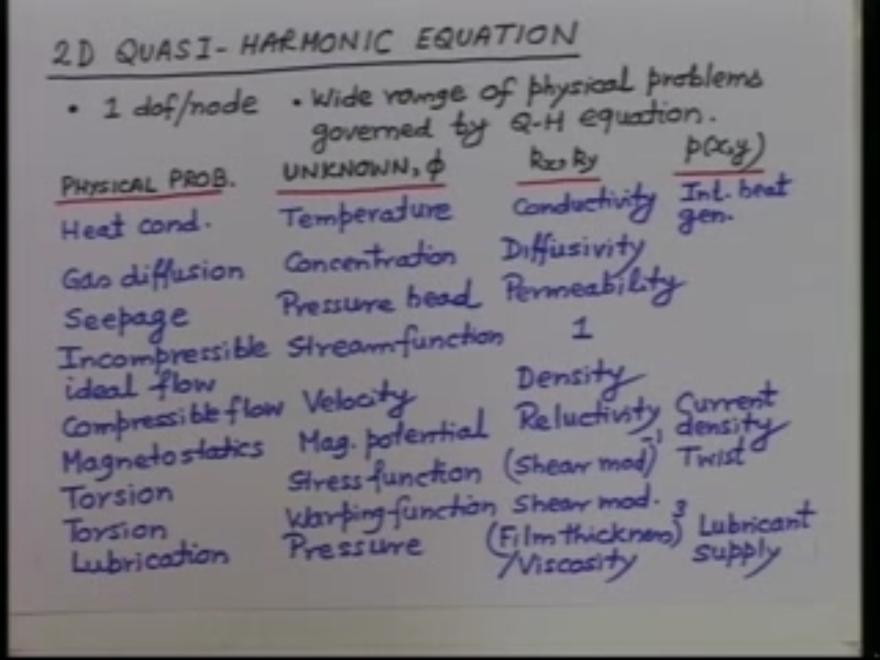
\includegraphics[width=0.7\linewidth]{../Notes_figure/nfem/fig7}
		\end{figure}
	\end{frame}


	
	\begin{frame}
		\begin{itemize}
			\item So $R(x,y) = k \frac{\partial^2 \phi}{\partial x^2} + k \frac{\partial^2 \phi}{\partial y^2} + p$
			\item Global error  =  $\sum_{e=1}^N  \int_{\Omega_e}local$
			\item WRM 
			\begin{equation}
				\int \int_{\Omega} W   \left( k \frac{\partial^2 \phi}{\partial x^2} + k \frac{\partial^2 \phi}{\partial y^2} + p \right) dx dy = 0  \qquad( Strong statement)
			\end{equation}
			\item Greens theorem : 
			\begin{equation}
				\int \int_A \left( \frac{\partial C}{\partial x} \frac{\partial D}{\partial x} - C \frac{\partial^2 D}{\partial x^2} \right) dA =  \int_S C \frac{\partial  D}{\partial x} L_x ds
			\end{equation}
			So we use this we get :
			\begin{equation}
				\int \int_A C \frac{\partial^2 D}{\partial x^2}  dA =  
				\int \int_A \frac{\partial C}{\partial x} \frac{\partial D}{\partial x} - 
				\int_S C \frac{\partial  D}{\partial x} L_x ds
			\end{equation}
			The first term is like $W(k \frac{\partial^2 \phi}{\partial x^2})$
		\end{itemize}
	\end{frame}


	\begin{frame}
		\begin{itemize}
			\item $\int \int_A  \frac{\partial W}{\partial x} k\frac{\partial \hat{\phi}}{\partial x} dA - \int_S W.k \frac{\partial \hat{\phi}}{\partial x} L_x ds + \int \int_A  \frac{\partial W}{\partial y} k\frac{\partial \hat{\phi}}{\partial y} dA - \int_S W.k \frac{\partial \hat{\phi}}{\partial y} L_y ds + \int \int W p dA = 0 $ (Weak statement)
			\item Where $L_x$ is direction cosine of s with respect to x
			\item $\hat{\phi} = \sum_{i=1}^{n}N_i(x,y)\phi_i$ (Ritz, bubonov)
			\item For $j^{th}$ node \\             $\int\int _A \frac{\partial N_j}{\partial x} k \frac{\partial \sum_{i=1}^{n} N_i \phi_i}{\partial x} dA - \int_S N_j k \frac{\partial \sum_{i=1}^{n} N_i \phi_i}{\partial x} L_x ds +
			\int\int _A \frac{\partial N_j}{\partial y} k \frac{\partial \sum_{i=1}^{n} N_i \phi_i}{\partial y} dA - \int_S N_j k \frac{\partial \sum_{i=1}^{n} N_i \phi_i}{\partial y} L_y ds + \int \int_A N_j p dA= 0 $
			\item So $K_{ij} = \int\int_A k \left( \frac{\partial N_i}{\partial x}\frac{\partial N_j}{\partial x} + \frac{\partial N_i}{\partial y}\frac{\partial N_j}{\partial y}\right)dA$
			\item $\ve{K  d= P + X_i (Direct)+ Newman } = F$	
	\end{itemize}
	\end{frame}



	\begin{frame}{Triangular element}
		\begin{itemize}
			\item Anticlockwise noded. Each node has (x,y)
			\item $\hat{\phi} = N_1(x,y)\phi_1+N_2(x,y)\phi_2+N_3(x,y)\phi_3$
			\item Let $\hat{\phi} = a + bx + cy$ (Three unknowns, you need three for a plane)
			\item $\mat{\phi_1;\phi_2;\phi_3} = \mat{1,x_1,y_1;1,x_2,y_2;1,y_2,y_3} \mat{a;b;c}$
			\item Then we can find the shape functions
			\item Then we can find the element! Stress and strain is constant
		\end{itemize}
	\end{frame}



	\begin{frame}{Quasi Harmonic problem}
		\begin{itemize}
			\item In plane deformation : Plane stress, plane strain, axisymmetric
			\item Integration over the triangle domain (area) poses problems
			\item Then they developed area coordinates, which is the area sections that they develop for the shape functions $L_i = N_i$. Some area integration based on these area coordinates.
			\item The stiffness is constant, and area can be formed while the force can be found
			
		\end{itemize}
	\end{frame}
 


	\begin{frame}
		The steps of a finite element method are
		\begin{itemize}
			\item Divide the whole domain ino finite parts
			\item For each element develop relations between pairs of dual variables (primary and secondary, eg forces and displacements)
			\item Assemle elements together to get the replationship of the variables for the whole system	
		\end{itemize}
		We are going to look at second differential equations and how to solve them using fem
	\end{frame}


	\begin{frame}{Example of primary and secondary variables}
		\begin{figure}
			\centering
			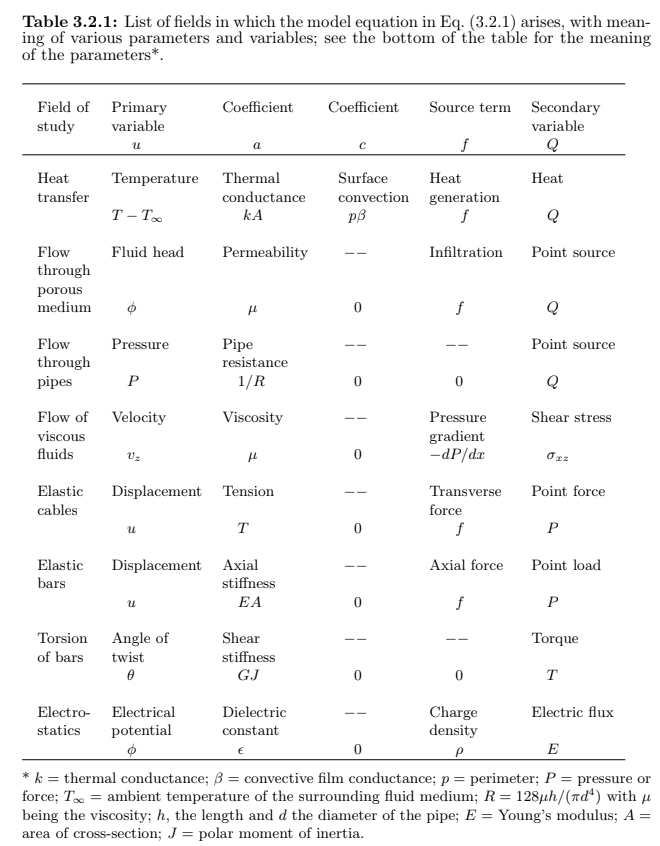
\includegraphics[width=0.5\linewidth]{\pth/nfem/fig2} 
		\end{figure}
	\end{frame}


	\begin{frame}{One-D Problem}
		\begin{itemize}
			\item Consider the equation
			\begin{equation}
				-\frac{d}{dx}\left(a \frac{u}{x} \right) + cu =  f \qquad for \qquad 0<x<L
			\end{equation}
			\item where $a = a(x), c = c(x), f = f(x)$ are the known quantities and $u(x)$ has to be found		
		\end{itemize}
	\end{frame}


	\begin{frame}{FEM approximation}
		\begin{itemize}
			\item The domain $\Omega = (0,L)$ is descritised into a set of intervals with $\Omega^e = (x_a^e,x_b^e)$ which denotes the end of the element 
			\item  The length of an element $h_e =x_b^e- x_a^e$
			\begin{figure}
				\centering
				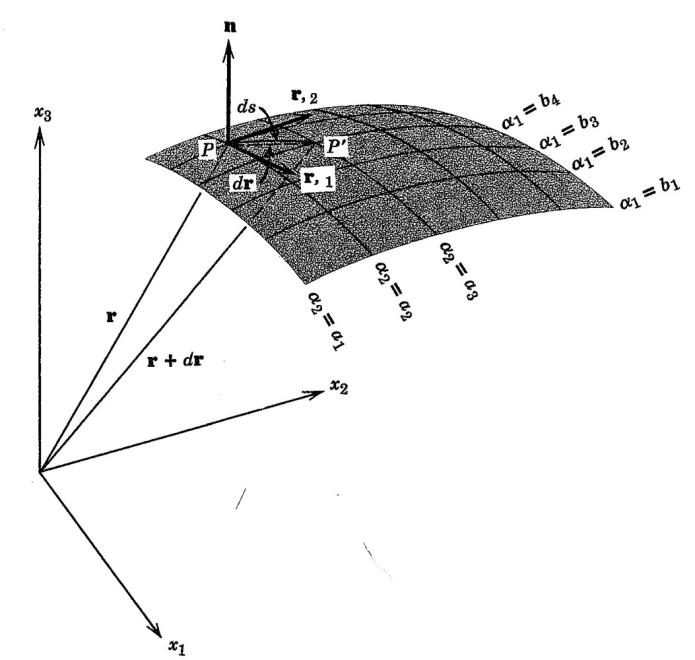
\includegraphics[width=0.7\linewidth]{\pth/nfem/fig1} 
			\end{figure}
			\item We find an approx solution over each element $\Omega^e$ and then we assemble it all together
			\begin{equation}
			u(x) \approx u_h^e(x) = \sum_{j}^{n}c^e_jN_j^e
			\end{equation}
			where we choose the shape functions and then have to find the coefficients such that oour approx solution is like the real one
			\item Since there are n unkown parameters (For each dof), we need n linearly independant equations

		\end{itemize}
	\end{frame}



	\begin{frame}{Discretised DE equation}
		\begin{itemize}
			\item Keeping the discretised DE equation we get 
				\begin{equation}
					-\frac{d}{dx}\left(a \frac{u_h^e}{x} \right) + cu_h^e -f(x) =  R^e(x,c_1^e,c_2^e,c_3^e,...,c_n^e) \neq 0  
				\end{equation}
			What we want to do is find the coefficients such that the residual is zero. This is again equilibirum at a point!
			\item One way to make it zero is to set the weighted integral of the residual zero
				\begin{equation}
					\int_{x_a^e}^{x_b^e} w_i^e(x)R^e(x,c_1^e,c_2^e,c_3^e,...,c_n^e)  dx = 0 \qquad i = 1,2,...,n
				\end{equation}
			\item where $w_i^e$ are different weight functions giving us n equations for the coefficien parameters ($c_1^e,c_2^e,c_3^e,...,c_n^e$)
			\item Now the weights however shoul all be independent and invertible. If we took w = 1, we would have only one equation
			\item These weights feel like the variation, but in the variation we choose also that the variations are the same function like the shape functions hmmmm.
		\end{itemize}
	\end{frame}


	\begin{frame}
		\begin{itemize}
			\item If we choose $w^e_i$ to be the shape functions. We get the Galerkin method. Which is exactly the same as the virtual work where $\delta v = \sum_{i}\delta v_i N_i$ where you can say then that $\delta v_i$ is 1, since the virtual disp magnitude comes out anyways
			\item Since the residual $R_e$ has the same order derivatives of the dependant unkonw u(x), we need at least quadratic representation of $u_h^e(x)$
			\item To reduce or weaken the differentiability of the shape functions (node disp are constant) , we distribute the order between the weights and $u_h^e$ 
			\begin{block}{}
				This is the weak form : Reducing the order of the dependant variable to the weight to make the order of the variable leser
			\end{block}
			\item The weights kind of give different component equilib equations
		\end{itemize}
	\end{frame}


	\begin{frame}{Note}
		\begin{itemize}
			\item Note that in usual structural mechanics we derive the virtual work equation from a potentional functional. Most fem methodsa re based on an element wise application of the Ritz method
			\item The virtual displacement is an integral statement which is he same as the integral weak form found frm the governing differential equations. 
			\item But differential equations are easy to form, and most fem methods are based on de
			
		\end{itemize}
	\end{frame}


	\begin{frame}{Derivation of the weak form}
		\begin{itemize}
			\item After getting the weighted residual statement, the next job is to weaken the  differentiability of $u_h^e$. To make both the orders of $u_h^e$ and $w_i^e$ the same
			\item The steps are 
			\begin{itemize}
				\item Write weighted residual statement
					\begin{equation}
						0 = \int_{x_a^e}^{x_b^e} \left[w_i^e\left(-\frac{d}{dx}\left(a \frac{u_h^e}{x} \right) + cu_h^e -f(x) \right) \right] dx
					\end{equation}
					We are taking the summation of the weighted residual over the whole element and saying that it is zero. The weight sort of gets the components
				\item Weakening the form using integration by parts
				\begin{equation}
					\begin{aligned}
					(uv)' = uv' + u'v \\
					\int_{a}^{b} uv' = uv|^b_a - \int_{a}^{b} u'v \\
					0 = \int_{x_a^e}^{x_b^e} \left[w_i^e\left(-\frac{d}{dx}\left(a \frac{u_h^e}{x} \right) + cu_h^e -f(x) \right) \right] dx\\
					0 = \int_{x_a^e}^{x_b^e} \left( a\frac{d w_i^e}{dx} \frac{du_h^e}{dx}  + cw^e_iu_h^e -w_i^ef(x) \right)  dx
					-\left[ w_i^e a \frac{du_h^e}{dx}\right]_{x_a^e}^{x_b^e}
					\end{aligned}
				\end{equation}
				
			\end{itemize}
			
		\end{itemize}
	\end{frame}


	\begin{frame}
		\begin{itemize}
			\item Very interesting, we actually get the boundary terms too!
			\begin{equation}
			0 = \int_{x_a^e}^{x_b^e} \left( a\frac{d w_i^e}{dx} \frac{du_h^e}{dx}  + cw^e_iu_h^e -w_i^ef(x) \right)  dx
			-\left[ w_i^e. a \frac{du_h^e}{dx}\right]_{x_a^e}^{x_b^e}
			\end{equation}
			Direct boundary on the dependant: Dritchlet/essential $u = 0$ \\
			Boundary on the derivatives of dependant : Newman/natural $\frac{du}{dx} = p$
			\item The coefficient of the weight function which is $a\frac{du}{dx}$ is the second variable
			\item We state the differenet variables
			\begin{equation}
			\text{Primary variable : } u\qquad \text{Secondary variable:} n_x(a\frac{du}{dx}) = Q(x)
			\end{equation}
			See that $n_x = -1,1$ on left and right end. ???WHye
			\item In the final weak form, we keep the secondary variables at the element ends as
			\begin{equation}
			Q_a^e = Q(x_a^e) = -\left(a \frac{du}{dx} \right)_{x_a^e} \qquad 	Q_b^e = Q(x_b^e) = \left(a \frac{du}{dx} \right)_{x_b^e}
			\end{equation}
			In the figure above we can think this of a FBD but in arbitary configruaion. The first one is a compressive, while later is a tensile force. In heat the first would be the heat input and later output
			\item Althout Q replaced $a(\frac{du}{dx})$, it is not consdiered as a function of u, but a variable dual to u??????
		\end{itemize}
	\end{frame}


	\begin{frame}{Final expresion}
		\begin{itemize}
			\item The final expression for the weak form is 
			\begin{equation}
				0 = \int_{x_a^e}^{x_b^e} \left( a \frac{d w_i^e}{dx}\frac{du_h^e}{dx}  + cw^e_iu_h^e -w_i^ef(x) \right)  dx
				- w_i^e(x_a^e)Q_a^e - w_i^e(x_b^e)Q_b^e
			\end{equation}
			But even in the virtual work when you reduce the order of the strains, you get the boundary condition
			\item The remarks are:
			\begin{itemize}
				\item Integration by parts (i) reduces the degree of the fem approximation (ii) introduces the secondary variables that are physically meanifull as they can be specified at a point where the primary variable is not specified. If the secondary variable is not a physical quantity, then the integraion by parts should not be carried out even to reduce the order of $u_h^e$
				\item The terms containing both $w_h^e$ and $u_h^e$ are called bilinear functional 
				\begin{equation}
					B(w_i^e,u_h^e) = \int_{x_a^e}^{x_b^e} \left(a \frac{d w_i^e}{dx}\frac{du_h^e}{dx} + cw^e_iu_h^e \right)
				\end{equation}
				but has to be linear with respect to $w_i^e$ and $u_i^e$. So it has to be billinear map. Like a scalar product with metric tensor where u and v are the input and the metric tensor is the bilinear map. If a or/and c is a fucntion of u. Then B is always linear in w but not u.
				\item Terms having only $w_i^e$ are only linear functionals because they are only linear with respect to $w_i^e$. $l(w_i^e)$
				
			\end{itemize}
		\end{itemize}
	\end{frame}


	\begin{frame}
		\begin{itemize}
			\item Therefore the weak form can be expressed as 
			\begin{equation}
				B(w_i^e,u_h^e) = l(w)i^2
			\end{equation}
			which is a vairational problem where we find $u^e \in U$ such that the equation is satisfied for all $w_i^e \in U$ (See Reddy page 103 for hilbert spaces)
			\item  The weak form is nothing but the statement of minimum total potential energy, or the variational minimum 
			\begin{equation}
				\begin{aligned}
					\Pi(u_h^e) \\
					\delta \Pi = B(\delta u_h^e,u_h^e) - l(\delta u_h^e) = 0 \\
					\Pi(u_h^e) = \frac{1}{2}B(\delta u_h^e,u_h^e) - l(\delta u_h^e) \\
					= \int_{x_a^e}^{x_b^e} \left[\frac{a}{2} \left(\frac{d u_i^e}{dx} \right)^2 + \frac{c}{2}(u_h^e)^2 - u_h^e f \right]dx - u_h^e(x_a^e)Q_a^e  - u_h^e(x_b^e)Q_b^e 
				\end{aligned}
			\end{equation}
			This is when you have reduced the order of the derivative in the virtual work, (We get the Euler lagrange equilibrium).
			\item This equation $\frac{1}{2}B(w_i^e,u_h^e) = l(w)i^2$, B shoudl be symmetric and the first term is the elastic energy while the later is the work done by the load and point loads.
		\end{itemize}
	\end{frame}


	\begin{frame}{Approximate functions}
		\begin{itemize}
			\item We have to satisfy the weak form of the differential equation along with the continuity and boundary conditions. We need to choose a function that satisfies the differntiability requirement and the end conditions $u(x_i) = u^e_i$.
			Any function with a non zero differentiation of the order of the weak form would be a candidate. We can therefore use interpolation.
			\item The interpolation is
			\begin{equation}
				u^e_h(x) = c_1^e + c_2^e x
			\end{equation}
			is okay, since the differentiation $\neq 0$, but we only now need to make sure that $c_1, c_2$ are such that the end displacements match
			\begin{equation}
				u^e_h(x_a^e) = c_1^e + c_2^ex_a^e = u_a^e \qquad
				u^e_h(x_b^e) = c_1^e + c_2^ex_b^e = u_b^e
			\end{equation}
			or \\
			$\mat{1,x_a^e;1,x_b^e} \mat{c_1^e;c_2^e} = \mat{u_a^e;u_b^e}$
			and we get the interpolating functions $u_h^e(x) = \sum_{j=1}^{2} N_j^eu_j^e$ \footnote{The book makes $\phi$ for N. But I usually use that for eigen directions?} 
			\item $N_1^e(x) = \ \frac{x_b^e-x}{x_b^e-x_a^e}$ \qquad $N_2^e(x) = \ \frac{x-x_a^e}{x_b^e-x_a^e}$
		\end{itemize}
	\end{frame}

	
	\begin{frame}
		\begin{figure}
			\centering
			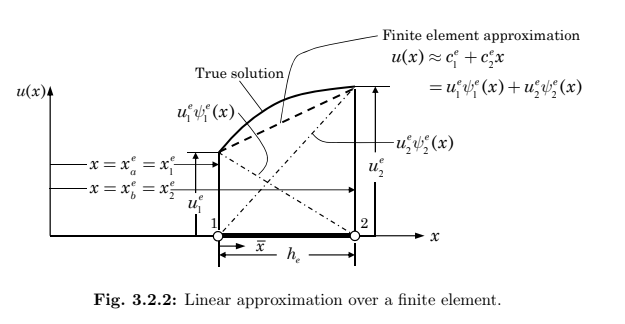
\includegraphics[width=0.7\linewidth]{\pth/nfem/fig3} 
		\end{figure}
		\begin{itemize}
			\item These N are linear lagrange interpolation functions and $u_1^e = u_a^e \qquad u_2^e = u_b^e$ are the nodal values of the approx function at the ends. $U_h$ belongs to a hilbert subspace spanned by $N_1^e,N_2^e$
			\item Remember that $N_i^e(x^e_j) = 1 \quad \text{if} i=j$. They also satisfy the partition of unity where $\sum_{j=1} N_j^e(x) =1$
			
		\end{itemize}
	\end{frame}


	\begin{frame}{Quadratic approxiamtions}
		For a quadratic approximation we choose
		\begin{equation}
			u_h^e(x) =  c_1^e + c_2^ex + c_3^ex^2
		\end{equation}
		\begin{itemize}
			\item Since there are three parameters we need to have three nodal points where we can relate the constants to. 
			\begin{equation}
				x_1^e =  x_a^e \qquad x_2^e =  x_a^e + \frac{h_e}{2} \qquad x_3^e = x_a^e + h_e = x_b^e
			\end{equation}
			And we similary get :
			\begin{equation}
				u_h^e(x) = \sum_{j=1} N^e_ju_j^e
			\end{equation}
			where $N$ are the quadratic lagrange interpolation functions. If they are expressed in local coordinate we get
			\begin{equation}
				N_1^e(x') = \left(1-\frac{x'}{h_e} \right)\left(1-\frac{2x'}{h_e} \right) \qquad N_2^e(x') =4\frac{x'}{h_e}\left(1-\frac{x'}{h_e} \right) \qquad N_3^e(x') = -\frac{x'}{h_e}\left(1-\frac{2x'}{h_e} \right) 
			\end{equation}
		\end{itemize}
	\end{frame}

	\begin{frame}
		\begin{figure}
			\centering
			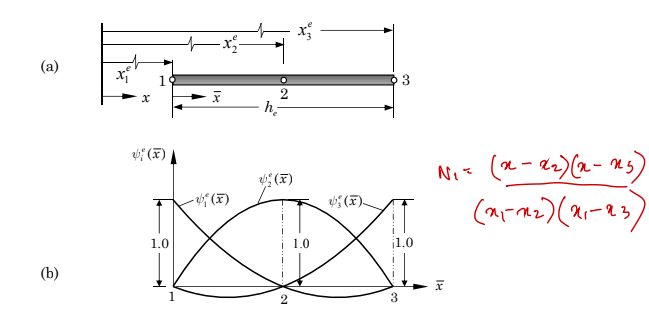
\includegraphics[width=0.7\linewidth]{\pth/nfem/fig4} 
		\end{figure}
		\begin{itemize}
			\item This is a quadratic element
			\item Any higher order lagrange interpolations can be developed. A (n-1)degree can be written as $u_h^e \sum_{j=1}^{n} N_j^eu_j^e$
			\item Where the interpolating function can be given as
			\begin{equation}
				N_j^e(x) = { \Pi_{i=1,i\neq j}} \left( \frac{x-x_i^e}{x_j^e-x_i^e} \right)
			\end{equation}
			For example $N_1(x) = \left(\frac{x-x_2}{x_1-x_2} \right)\left(\frac{x-x_3}{x_1-x_3} \right)$
		\end{itemize}
	\end{frame}


	\begin{frame}{Comments}
		\begin{itemize}
			\item Approx solution should be continous and differentiable as needed by the weak form. This ensures that every term in the differential equaion does not have a zero coefficient.
			\item It should be a complete polynomial (Pascal's law). To capture all the actual deformation. Lower to higher!
			\item It should interpolate the primary variables at the nodes of the fem and at the end points. To ensure continuity of the primary variable acorss elements!		
			
		\end{itemize}
	\end{frame}


	\begin{frame}{FEM model}
		\begin{itemize}
			\item Keeping the approximate solutions in the weak form gives us the algebraic equatins
			\item The degree of the approx solution has to be decied a priori. If there are more than 2 nodes, then the number of non-zero secondary variables increases at the interior nodes
			\begin{equation}
				 0 = \int_{x_a}^{x_b} \left(a \frac{dw_i^e}{dx} \frac{du_h^e}{dx} + cw_i^eu_h^e\right)dx - \int_{x_a}^{x_b} w_i^ef dx - \sum_{j=1}^{n} w_i^e (x_j^e)Q_j^e
			\end{equation}
			\item If 1 and n denote the end points then $Q_1^e,Q_n^e$ denote the unknown point sources, while the other $Q_j^e \quad(j=2,3...n-1)$ are the externally applied and known point sources. So at the ends these are internal or external loads??????
			\item If we keep $w_i^e = N_i^e$ into the weak form, we get n algebraic equations. This is the Galerkin  method (Original was weighted of residual and not of the weak form, that would be exactly the same to Ritz method). The $i$th algebraic equation is the one obtained by keeping $w_i^e$ as $N_i^e$. This is the same as the virtual work method, where each equation of a discretised system comes from the virtual displacement of each node 
		\end{itemize}
	\end{frame}


	\begin{frame}
		\begin{itemize}
			\item So we get
			\begin{equation}
				 0 = \int_{x_a}^{x_b} \left(a \frac{dN_i^e}{dx} \sum_{j=1}^{n} u_j^e\frac{dN_j^e}{dx} + cN_i^e\sum_{j=1}^{n}u_j^eN_j^e\right)dx - \int_{x_a}^{x_b} N_i^ef dx -  \sum_{j=1}^{n} N_i^e (x_j^e)Q_j^e
			\end{equation}
			so for each equation i there will be a summation on the derivatives of the approx solution due to chain rule! and we get
			\begin{equation}
				 0 = \sum_{j=1}^{n} \left[ \int_{x_a}^{x_b} \left(a \frac{dN_i^e}{dx}  \frac{dN_j^e}{dx} + cN_i^e N_j^e\right)dx\right]u_j^e - \int_{x_a}^{x_b} N_i^ef dx -  Q_i^e
			\end{equation}
			where we have taken the summation of u magitude coefficient for, shape functions  outside. Also we see that for each shape function at each node we actually only get the boundary load at that variation. Because $N_i^e(x^e_j) = 0$ when $i \neq j$. We get for each node!
			\begin{equation}
				0 = \sum_{j=1}^{n} K_{ij}^e u_j^e - f_i^e - Q_i^e
			\end{equation}
		\end{itemize}

	\end{frame}

	\begin{frame}
		\begin{itemize}
			\item Where
			\begin{equation}
			\begin{aligned}
				K_{ij}^e = \int_{x_a}^{x_b} \left(a \frac{dN_i^e}{dx}  \frac{dN_j^e}{dx} + cN_i^e N_j^e\right)dx  =  B(N_i^e,N_j^e)\\
				f_i^e = \int_{x_a}^{x_b} fN_i^e dx = l(N_i^e)
			\end{aligned}
			\end{equation}
			So this is ineresting the coefficient of the stifness says basically states chagne in the shape functions!
		\end{itemize}
		\begin{block}{Matrix form}
			\centering
			$\ve{K^eu^e = f^e + Q^e \approx F^e}$
		\end{block}
	where 
		\begin{itemize}
			\item $K^e$	is the symmetric coefficient, stiffness matrix
			\item $f^e$ is the source or force vector
			\item This method is the weak-form Glaerikin or Ritz finite element method
		\end{itemize}
	
	\end{frame}


	\begin{frame}
		\begin{block}{Matrix form}
			\centering
			$\ve{K^eu^e = f^e + Q^e \approx F^e}$
		\end{block}
		\begin{itemize}
			\item But for every element, we have $n$ equations and $n+2$ unknowns. The 2 unkowns are the secondary nodal values that we don't know $Q_a^e, Q_b^e$. ($u_1^e,u_2^e...u_n^e$) are the element primary nodal degrees. Remember these values, we know if they are along the inside of the element as external forces. 
			\item Assembling the elements by imposing the continuity of the elements. U2 of 1 is U1 of 2. We get the same number of equations and unkowns (Primary + Secondary). 
			\item The stiffness and force matrix can be found for a certain value. And if the coefficients (a,c,f) are also functions of x, then we need to do numerical integration. 
		\end{itemize}
	\end{frame}


	\begin{frame}{General fem one-d matrix form}
		\begin{figure}
			\centering
			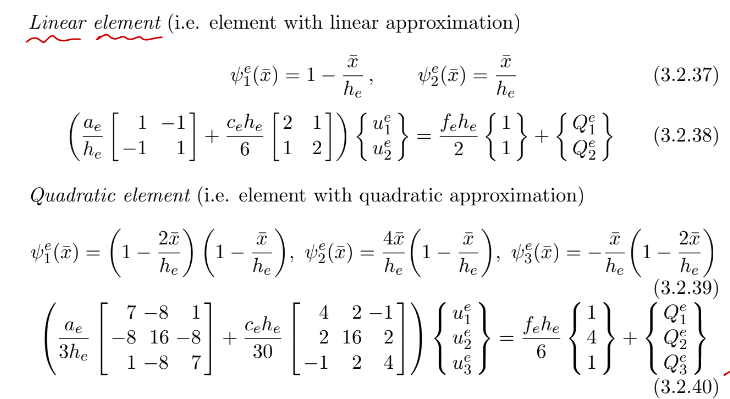
\includegraphics[width=0.7\linewidth]{\pth/nfem/fig5} 
		\end{figure}
	
	     \begin{itemize}
	     	\item Where in linear element lets write the expansion for the first linear element equation
	     	\begin{equation}
	     	\tiny
	     	\begin{aligned}
	     		    K_{11}u_1^e + K_{12}u_2^e = {f_1} + Q_1^e \\ 
	     		    \left[\int_{0}^{h_e} a\frac{-1}{h_e}\frac{-1}{h_e} + c\left(1-\frac{x}{h_e} \right)\left(1-\frac{x}{h_e} \right) \right] u_1^e 
	     		    + \left[\int_{0}^{h_e} a\frac{-1}{h_e}\frac{1}{h_e} + c\left(1 -\frac{x}{h_e} \right)\left(\frac{x}{h_e} \right) \right] u_2^e  =  \int_{0}^{h_e} f\left(1-\frac{x}{h_e} \right) + Q_1^e 
	     	\end{aligned}
	     	\end{equation}
	     	\footnote{ We note that (i) In quad, the force vector is not just fh/3 but it depends on the work done! Not same with 2 elements combined. (ii) There are also more unkowns thatn the no of equations. When one element is used however we have only n unkowns cause bcs will be applied on Q.}  
	     \end{itemize}
	\end{frame}


	\begin{frame}{Problem \#1}
		\begin{itemize}
			\item Consider a homogeneous, isotropic bar of length L(m), cross sectional area (A) and conductivity k (W/($m^oC$))
			\item  Ambient temperature is $T_o(^oC)$
			\item No heat loss throughout the bar and the right end is exposed to ambient temperature of $T_{inf }$
			\item Uniform heat of $g_o$, heat transfer with fin and air is $\beta$
			\item Check Reddy Page 3.2.1
		\end{itemize}
		\begin{figure}
			\centering
			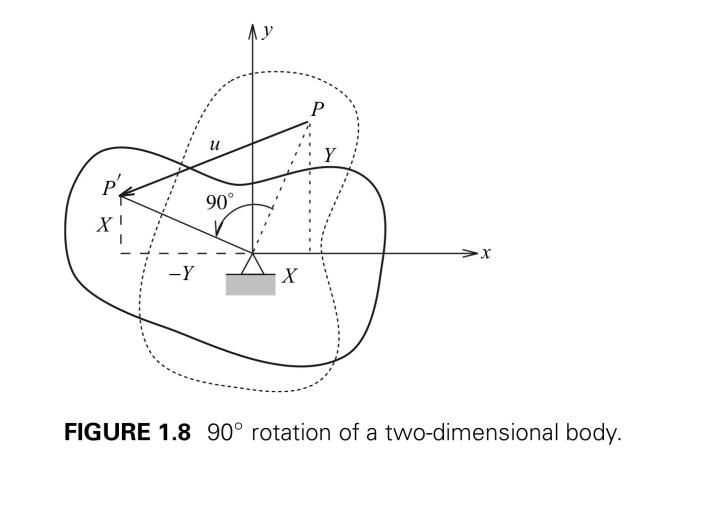
\includegraphics[width=0.7\linewidth]{\pth/nfem/fig6} 
		\end{figure} 
	\end{frame}


	\begin{frame}
		\begin{figure}
			\centering
			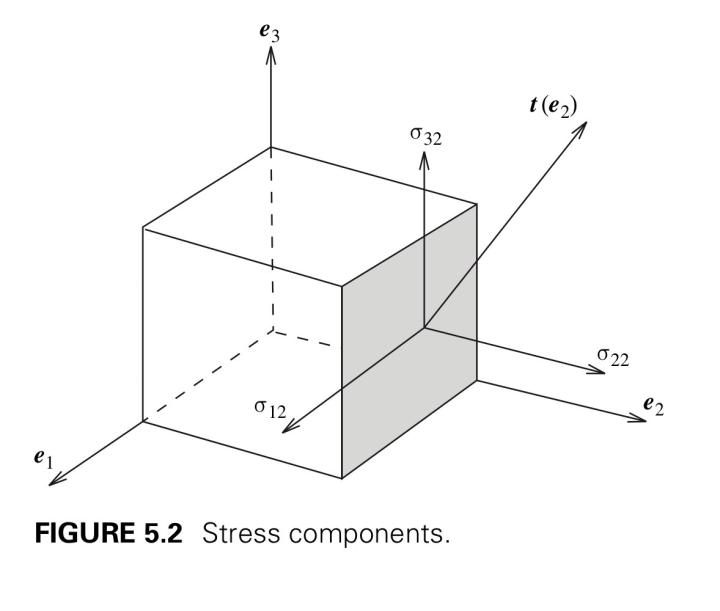
\includegraphics[width=0.7\linewidth]{\pth/nfem/fig8} 
		\end{figure} 
		\begin{itemize}
			\item Remember when we draw the internal force signs as compressive for a tensile element. This we are drawing for the nodal equilibrium side cut of the fbd. Rembember force, stresses are all defined with respect to the cut and face. 
			\item In the Reddy example you will find that at the B.C., the internal force reaction at the node, $Q^4_2$ and $kU_5$ is a force in $\leftarrow$
		\end{itemize}
	\end{frame}



	\begin{frame}{Natural coordinates}
		\begin{itemize}
			\item Check reddy 114 for origin at left side of element, natural $\bar{x}$
			\item Origin at center denoted as $\xi$
				\begin{itemize}
					\item $\xi$ is -1 and +1 at LHS and RHS. Since your current basis is eucledian. The transfromation is linear.
					\item x can be given as a function of $\xi$ and found out
					\item This is interesting. Suppose $x = x_a +\frac{h}{2}(1+\xi)$
					\begin{equation}
					\begin{aligned}
						\frac{d }{d x}  = \frac{2}{h}\frac{d }{d \xi} \quad \frac{d N_i}{d x}  = \frac{2}{h}\frac{d N_i}{d \xi} \\
						dx = \frac{h}{2} d\xi \\ 
						\int_{x_a^e}^{x_b^e}  N_i(x) dx = \int_{0}^{h}  N_i(\bar{x}) d\bar{x} = \frac{h}{2} \int_{-1}^{1} N_i(\xi) d\xi \\ 
						\int_{x_a^e}^{x_b^e}  \frac{dN_i(x)}{x} dx = \int_{0}^{h}  \frac{N_i(\bar{x})}{\bar{x}} d\bar{x} =  \int_{-1}^{1} \frac{N_i(\xi)}{d\xi} d\xi \\ 
						\int_{x_a^e}^{x_b^e}  \frac{dN_i(x)}{x} \frac{dN_j(x)}{x} dx = \int_{0}^{h}  \frac{N_i(\bar{x})}{\bar{x}}  \frac{N_j(\bar{x})}{\bar{x}} d\bar{x} = \frac{2}{h} \int_{-1}^{1} \frac{N_i(\xi)}{d\xi} \frac{N_j(\xi)}{d\xi}d\xi 
					\end{aligned}
					\end{equation}	
				\end{itemize}
			
		\end{itemize}
	\end{frame}



	\begin{frame}{2D problems}
		\begin{itemize}
			\item Governing differential equation. Suppose a single field $u(x,y)$ with the following partial differential equation  varies over x and y
			\item $\frac{\partial }{\partial x} \left(k_x\frac{\partial \phi}{\partial x} \right) + \frac{\partial }{\partial y} \left(k_y\frac{\partial \phi}{\partial y} \right) + f(x,y) = 0$
			where for a heat problem, k is the conucitvity in a orthotropic medium and u is the temperature and f is the internal heat generation.  
			\item Mixed boundary conditions 
			\begin{itemize}
				\item Dritchlet : $\phi = \hat{\phi}$ in some boundary
				\item General Newman :$k_x\frac{\partial u}{\partial x} n_x  + k_y\frac{\partial u}{\partial y} n_y + q_c =  \hat{q_n}$ : In some portion of the boundary. 
				\begin{itemize}
					\item $q_c$ represents the convective component of flux (heat problems $q_c = h_c(u-u_c)$)
					\item $n_x = cos(x,\ve{n})$ and $n_y = cos(y,\ve{n})$ which is the angle of the normal of the boundary and the axis
					\item $u_c$ is the ambient temperature and $h_c$ is the convective heat coefficient				
				\end{itemize}		
			\end{itemize}
		\end{itemize}
	\end{frame}


	\begin{frame}{FEM approximation}
		\begin{itemize}
			\item In FEM the domain is descritised into subdomains. Any shape qualifies as long as the approximating functions $N_i^e$ can be derived uniquely for the shape. The discretisation may be may not represent the actual boundary though at really curved regions.
			\item Suppose the dependent unkown $u$ is given by $\hat{u^e} = \sum_{j=1}^{n} u_j^eN_j^e(x,y)$
			\item The interpolation functions depend not only on the number of nodes but also on the shape of the element
			\item A triangle will need two points given by $\hat{u^e} = c_1+c_2x+c_3y$
			\item A triangle with three nodes in each side is given by $\hat{u^e} = c_1+c_2x+c_3y + c_4xy + c_5x^2 + c_6y^2$			
		\end{itemize}
	\end{frame}



	\begin{frame}{Weak form}
		\begin{itemize}
			\item The n nodal values $u_j^e$ must be found such that the approximating solution $u_h^e(x)$ satisfies the governing differential equation in a weak sense. Steps are :
			\begin{enumerate}
				\item Take non zeros of the G.D.E as R(x,y) and multiply by the weight function $w_i^e$ from a set of linearly independant functions. We get then 
				\begin{equation}
				\int \int_{\Omega} w_i^e  \left( k \frac{\partial^2 u_h^e}{\partial x^2} + k \frac{\partial^2 u_h^e}{\partial y^2} - f(x,y) \right) dx dy = 0  \qquad( Strong statement)
				\end{equation} For n independant choices of $w_i^e$, we get n independant equations.
				\item Distribute so that for both $u_h^e, w_i^e$ are required to be differentiated once. Using component form of the divergence theorem or Greens theorem : 
				\begin{equation}
				\begin{aligned}
					\int \int_A \frac{\partial}{\partial x} (w_i^e F_1) dA = \int_S (w_i^eF_i)n_x ds   \\
					\int \int_A \frac{\partial}{\partial y} (w_i^e F_2) dA = \int_S (w_i^eF_i)n_y ds   \\
					F_1 = k_x \frac{\partial u^e_h}{\partial x} \qquad 
					F_2 = k_y \frac{\partial u^e_h}{\partial y}
				\end{aligned}
				\end{equation}
				And from product rule we get 
				\begin{equation}
					-w_i^e\frac{\partial F_1}{\partial x} = -\frac{\partial }{\partial x}(w_i^eF_1) + F_1 \frac{\partial w_i^e}{\partial x} 
					\qquad
					-w_i^e\frac{\partial F_2}{\partial x} = -\frac{\partial }{\partial x}(w_i^eF_2) + F_2 \frac{\partial w_i^e}{\partial x} 					
				\end{equation}		
			\end{enumerate}		
		\end{itemize}
	\end{frame}



	\begin{frame}
		\begin{itemize}
			\item And we get the weak form as \\
			$0 = \int\int_A   \left( k_x \frac{\partial w_i^e}{\partial x}\frac{\partial u_h^e}{\partial x} + k_y \frac{\partial w_i^e}{\partial x}\frac{\partial u_h^e}{\partial y} - w_i^ef(x,y) \right) dA - \int_S w_i^e \left( k_x \frac{\partial u_h^e}{\partial x}n_x + k_y \frac{\partial u_h^e}{\partial x}n_y \right) dS$
			\item Now the order of the differentiation has been reduced. 	
			\item Looking at the boundary terms, we see that $u_h^e$ is the primary variable and essential boundary. $q_n = \left( k_x \frac{\partial u_h^e}{\partial x}n_x + k_y \frac{\partial u_h^e}{\partial x}n_y \right)$ is the secondary variable and the natural boundary condition. It is positive as one travels counterclockwise in the boundary. 
			\item This is wy nodes are counted in counterclockwise and boundary integrals are carried in counter-clockwise sense. $\ve{q}$ is the outward flux normal and the flux $\ve{q} =q_x e_1 + q_ye_2 \qquad \qquad q_x= k_x \frac{\partial u_h^e}{\partial x}  \quad q_y = k_y\frac{\partial u_h^e}{\partial y}$
			\item  The normal flux is given by 
			\begin{equation}
			q_n = \hat{n}.\ve{q} =  k_x \frac{\partial u_h^e}{\partial x}n_x + k_y\frac{\partial u_h^e}{\partial y}n_y
			\end{equation}
		\end{itemize}
	\end{frame}



	\begin{frame}
		\begin{enumerate}
			\item So the third step is to use the general Newmann boundary condition and write as 
			\begin{equation}
			0 = \int\int_A   \left( k_x \frac{\partial w_i^e}{\partial x}\frac{\partial u_h^e}{\partial x} + k_y \frac{\partial w_i^e}{\partial x}\frac{\partial u_h^e}{\partial y} - w_i^ef(x,y) \right) dA - \int_S w_i^e \left( \hat{q_n} -h_c(u_h^e-u_c) \right) dS
			\end{equation}
			\item Rearragning we get 
			\begin{equation}
			0 = \int\int_A   \left( k_x \frac{\partial w_i^e}{\partial x}\frac{\partial u_h^e}{\partial x} + k_y \frac{\partial w_i^e}{\partial x}\frac{\partial u_h^e}{\partial y} - w_i^ef(x,y) \right) dA - \int_S h_cw_i^e u_h^e dS	- \int_S w_i^e \left( \hat{q_n} +h_cu_c \right) dS		
			\end{equation}
			\item So we get the form $B(w_i^e,u_h^e) = l(w_i^e)$
		\end{enumerate}
	\end{frame}


	\begin{frame}
		\begin{itemize}
			\item Note that the variational problem is to find a $u_h^e$ such that  $B(w_i^e,u_h^e) = l(w_i^e)$ for all $w_i^e \in U_h$ a subspace span by polynomial basis functions.
			\item $B(w_i^e,u_h^e) $ is bilinear and symmetric and $ l(w_i^e)$ is linear in w. So we can construct a functional $I = \frac{1}{2}B(u_h^e,u_h^e) -l(u_h^e)$ and the minmum is equivalent to solving the variation problem.
			\item It is not always possible to make a functional whose weak form  whose first variation is equivalent to the weak form. 
			
		\end{itemize}
	\end{frame}


	\begin{frame}{Finite element method}
		\begin{itemize}
			\item The weak form in the above equation requires that the approx function to be at least linear in both x and y. Suppose that $u_h^e = N_i u_i$
			\item The weak form is given as 
			\begin{equation}
			\begin{aligned}
				\left(\int\int _A \frac{\partial N_j}{\partial x} k \frac{\partial \sum_{i=1}^{n} N_i }{\partial x} dA +
				\int\int _A \frac{\partial N_j}{\partial y} k \frac{\partial \sum_{i=1}^{n} N_i }{\partial y} dA + \int_S h_c w_i^e N_j^e \right)u_j^e= 0 \\
				- \int_A N_i^ef dA - \int_S N_i^e(\hat{q}+h_cu_c)dS
			\end{aligned}
			\end{equation}	
			\item  This is when w is taken as the virtual displacemnt of the dependant unkown or $w_i^e = \delta u_h^e$. Each w we get a seperate equation and we get 
			\item $K^eu^e = f^e + q^e$
		\end{itemize}
	\end{frame}



	\begin{frame}{Approximating functions}
		\begin{itemize}
			\item u should be continous as required in the weak form that is all the terms are represented as non zero values
			\item  The polynomials must be complete and contain the same order of x and y
			\item All the terms in the polynomial should be linearly independant. The no o flinearly independent terms in represnetin u dictate the shape and no of nodes. It turns out only triangular and quad elements satisfy this.
		\end{itemize}
	\end{frame}




	\begin{frame}{Linear triangular element}
		\begin{itemize}
			\item The lowest order polynomial that we can come up with is
			\begin{equation}
			u_h^e(x,y) =c_1^e + c_2^ex +c_3^ey
			\end{equation}
			\item The set {1,x,y} is also linearly independant forming the basis for the subspace of the H1 hilbert space
			\item Now we need to find out a geometry that we can also use the continuity cnditions. And we get a triangle
			\item Check reddy 123 for shape functions
			\item  The shape functions are lagrange interpolation functions, with the sum =1
			\item If you mess up the aspect ratio, you will mess up the underlying physics. An intuition is as sometimes the stiffness can be decomposed to different matrixes that are dependant on its aspect ratio and the material properties.
			\item The boundary conditions $q$ are not found for elements connected on all sides, but with nodes on the boundary, $q_n^e$ is known and found by $q_i^e = \int_S \hat{q_n}N_i^e(s)dS$.  The internal boundary forces are canceled, like the balance of internal forces.
		\end{itemize}
	\end{frame}



	\begin{frame}{Linear bilinear (Lienar in x and y) rectangular element}
		\begin{itemize}
			\item The next polynomial that meets the requirements on the approx solution is 
			\begin{equation}
				u_h^e(x,y) =c_1^e + c_2^ex +c_3^ey + c_4xy
			\end{equation}
			\item  Th geometry is a quad element with a linear variation along two points in the element. We usually use isoparametric elements to represent the element.
			\item Also node is named counterclockwise.
			\item Reddy 126 for shape functions. Again we see that the aspect ration mess up the stiffness matrix. 
		\end{itemize}
	\end{frame}



	\begin{frame}{Higher order triangular element}
		\begin{itemize}
			\item For triangular elements, we can construct natural coordinates $L_i$
			\item $N_i = L_i = \frac{A_i}{A}$
			\item $\ve{N} = \mat{L_1(2L_1-1);L_2(2L_2-1);L_3(2L_3-1);4L_1L_2;4L_2L_3;4L_3L_1}$
			\item Formula to find the area also given using fromula (Reddy 128)
		\end{itemize}
	\end{frame}


	\begin{frame}{Higher order rectangular element}
		\begin{itemize}
			\item By multiplying from single linear we get four node
			\item Tensor product two quadratic one d we get quadratic quad element. 
			\item Serendipity have no interior node. Not complete. They don't have the dual$^2$ term. 
		\end{itemize}
	\end{frame}



	\begin{frame}{Element assembly}
		\begin{itemize}
			\item Continuity of primary variable : Same nodes from different elements
			\item Equilibrium of secondary variables : At the interface between two elements, the flux or internal force fro the two elements is equal and opposite in sign. 
			
		\end{itemize}
	\end{frame}



	\begin{frame}{Axisymmetric problem}
		\begin{itemize}
			\item   The same second order equation in the polar coordinates are given as 
			\begin{equation}
				\frac{1}{r}\frac{\partial }{\partial r}\left(r k_{rr} \frac{\partial u}{\partial r} \right)
				+ \frac{1}{r^2}\frac{\partial }{\partial \theta}\left( k_{\theta\theta} \frac{\partial u}{\partial \theta} \right)
				+ \frac{\partial }{\partial z}\left(k_{zz} \frac{\partial u}{\partial z} \right) + f(r,\theta,z)=0
			\end{equation}
			\item We can remove the terms of $z$ and $\theta$ as if the problem is independant of these parameters. 
			\item Reddy Page 137, One D and two D equations
		\end{itemize}
	\end{frame}



	\begin{frame}{Numerical integration}
		\begin{itemize}
			\item We use numerical integration. We use some parametric form to also do the integration on a square
		\end{itemize}
	\end{frame}


	\begin{frame}{Coordingate transforms}
		\begin{itemize}
			\item We do it on a square region dimension (2x2) with respect to ($\xi,\eta$) in domain -1< <1.
			\item The element of the fem mesh is transformed, only for the purpose of numerical integration. 
			\item We use a coordinate transformation of the form 
			\begin{equation}
			\begin{aligned}
				x = \sum_{j=1}^{m} x_j^e N_j^e(\xi,\eta) \qquad \qquad 				y = \sum_{j=1}^{m} y_j^e N_j^e(\xi,\eta) \qquad \qquad 
			\end{aligned}	
			\end{equation}
			\item The shape functions are of the master element in the -1 to 1 coordinate.
			\item  The master element is transformed in the linear transfmration to the quadrilateral element. 
			\item The dependant variable is also approximated by the same
			\begin{equation}
				u_h^e = \sum_{j=1}^{n} u_j^e \phi_j^e(\xi,\eta)
			\end{equation}
		\end{itemize}
	\end{frame}


	
	\begin{frame}
		\begin{itemize}
			\item Superparametric : If m > n. Geometry approx is higher
			\item Isoparametric : If m = n
			\item Subparametric : If m < n. If dependant variable is higher.
			
		\end{itemize}
		Transfomration of the quad to the master is for numerical evaluation. The final equations are alwayas in terms of the nodal values of the physical domain.
		\begin{enumerate}
			\item Different elements can be generated from the same master element. A master elemeent can have differnet order.
			\item A quad master can genreate quad curvilinear elements. 
			\item But elements should not overlap each other.
		\end{enumerate}
	\end{frame}



	\begin{frame}
		\begin{itemize}
			\item Consider the stiffness matrix 
			\begin{equation}
				K^e_{ji} =  \int\int _A \frac{\partial N_j}{\partial x} k_x \frac{\partial  N_i }{\partial x} dA +
				\int\int _A \frac{\partial N_j}{\partial y} k_y \frac{\partial N_i }{\partial y} dA
			\end{equation}
			\item Now this is in the global coordinates and we want to write it in terms of $\xi$ and $\eta$. 
			\item We can write using chain rule 
			\begin{equation}
				\mat{\frac{\partial N_i^e}{\partial \xi }; ;\frac{\partial N_i^e}{\partial \eta}} = \mat{\frac{\partial x}{\partial \xi},\frac{\partial y}{\partial \xi}; , ;\frac{\partial x}{\partial \eta},\frac{\partial y}{\partial \eta}}
				\mat{\frac{\partial N_i^e}{\partial x }; ;\frac{\partial N_i^e}{\partial y}}
			\end{equation}
			With the inner matrix the Jacobian $\ve{J}$, whose determinant should be >0
			\item We can then find the inverese transformation for the derivatives as $\ve{ N,_{(x,y)} = J^{-1}N,_{(\xi,\eta)}}$
			\item The geometry can also be easily differentiated
			\begin{equation}
			 \frac{\partial x}{\partial \xi} = \sum_{j=1}^{m} x_j^e \frac{\partial N_j}{\partial \xi} \quad \text{and so on}
			\end{equation}
		\end{itemize}
	\end{frame}



	\begin{frame}
		\begin{itemize}
			\item Obviously we also get $dA = det(J)\xi\eta$
			\item When all or some of the variables are approximated using hermite interpolating functions, linear approx of geometry and so subparametric or isoparametric forms are adopted.
			\item  Full stiffness matrix, we keep the terms in intergration in the master coodrinate. See Page 147
			\item Integration over a master element can also be looked at page 148 and 149. Itis basically $\int_{-1}^{1}\int_{-1}^{1} F(\xi,\eta) d\xi d\eta = \sum_{I=1}^{M} \int_{J=1}^{N} F(\xi_I,\eta_J) W_i W_j$
		\end{itemize}
	\end{frame}


\section{One D problem : Single variable}
	\begin{frame}
		\begin{itemize}
			\item A(u(x)) = f(x) in interval 0 <x<L $\qquad$ B(u) = g
			\item Consider the differential equation
			\begin{equation}
			\begin{aligned}
				-\frac{d}{dx}\left(k(x,u) \frac{du}{dx} \right) + b(x,u)\frac{du}{dx} + c(x,u)u = f(x) \quad 0<x<L \\
				\text{Boundary conditions}\\
				n_xk\frac{du}{dx} + \beta(x,u)(u-u_{\infty}) = \hat{Q}   \quad or \quad u = \hat{u}
			\end{aligned}
			\end{equation}
			\item Note that $n_x=-1, \beta = \beta_1$ at $x = x_a$ and $n_x=1, \beta = \beta_2$ at $x = x_b$
			\item For a bar with a spring, $u_{\infty} = 0$ and we get the equation that the bar should be equal to the spring force $\beta u$. Or $-k\frac{du}{dx}-\beta_2u = Q_2 $ where Q2 is the extrenal force.
			\begin{figure}
				\centering
				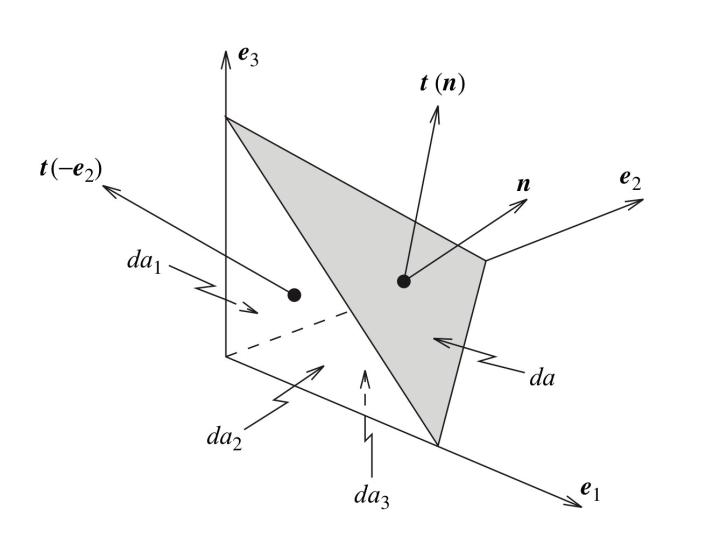
\includegraphics[width=0.7\linewidth]{\pth/nfem/fig9} 
			\end{figure} 
		\end{itemize}
	\end{frame}


	\begin{frame}
		\begin{itemize}
			\item Therefore we can keep it generally and nicely as:
			\begin{equation}
			\begin{aligned}
				A(u) = f \quad in \quad 0<x<L \qquad B(u) = g \quad at \quad x=0 or L \\
				A = -\frac{d}{dx}\left(a \frac{d}{dx} \right) +  \frac{d}{dx} + c. \quad B = n_x a \frac{d}{dx} + \beta, \quad g = \beta u_{\infty} + \hat{Q}
			\end{aligned}
			\end{equation}
			\item If a,b,c are functions of u then A and B become nonlienear.
			\item In heat a = kA, b = 0 and c = perimeter  $. \beta$
		\end{itemize}
	\end{frame}


	\begin{frame}{Weak formulation}
	\begin{figure}
			\centering
			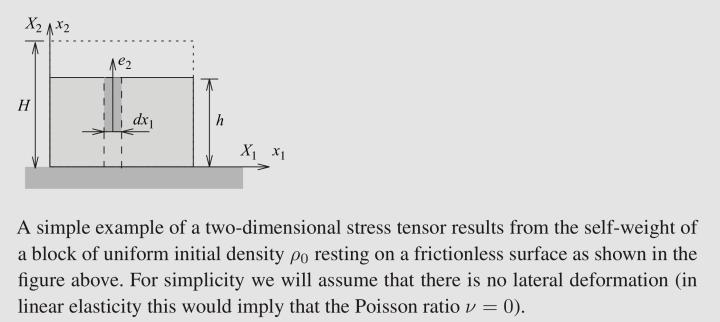
\includegraphics[width=0.7\linewidth]{\pth/nfem/fig10} 
		\end{figure}
	\end{frame}


	\begin{frame}{FEM}
		\begin{itemize}
			\item If we use the discretisation then we will get 
			\begin{equation}
			K(U)U = F
			\end{equation}
		\end{itemize} 
		\begin{figure}
		\centering
		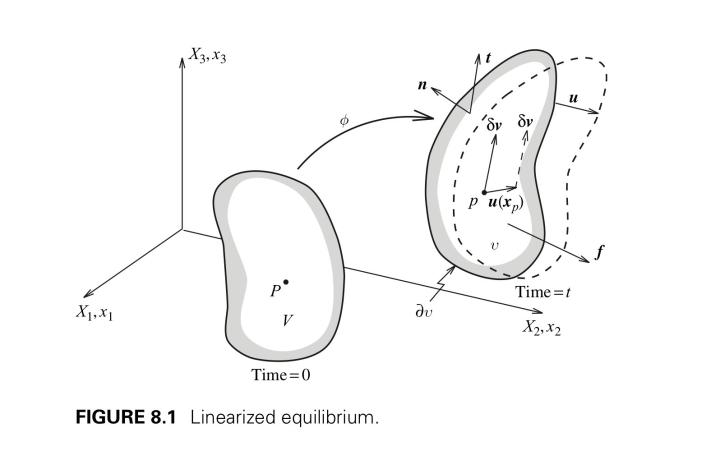
\includegraphics[width=0.8\linewidth]{\pth/nfem/fig11} 
		\end{figure}
	\end{frame}


	\begin{frame}
		\begin{itemize}
			\item The Boundary terms still confuses me. Especially the sign part. So here it is! Qe is the external force. F is the nodal force with equivalent parts. We actually get the external force from the internal Boundary terms!
			\begin{figure}
				\centering
				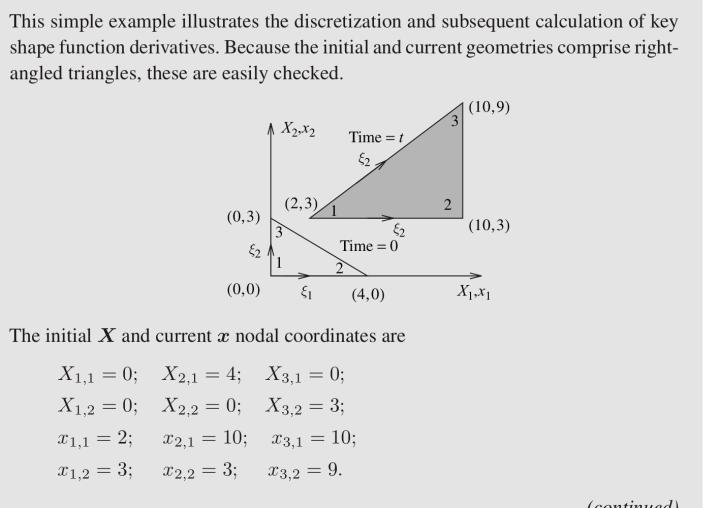
\includegraphics[width=1\linewidth]{\pth/nfem/fig12} 
			\end{figure}
			\item Check problem from Reddy for nonlinear constraints etc.
		\end{itemize}
	\end{frame}



	\begin{frame}{Solution of nonlinear algebrai equations	}
		\begin{itemize}
			\item Direct iteration procedure
			\item Newton rhapson method
		\end{itemize}
	\end{frame}


	\begin{frame}{Direct Iteration procedure}
		\begin{itemize}
			\item We solve this system of equations using direct iteration, Picard iteration or method of successive substitutions
			\begin{equation}
				\ve{K(U^{(r-1)})U^r = F(U^{(r-1)})}
			\end{equation}
			\begin{figure}
				\centering
				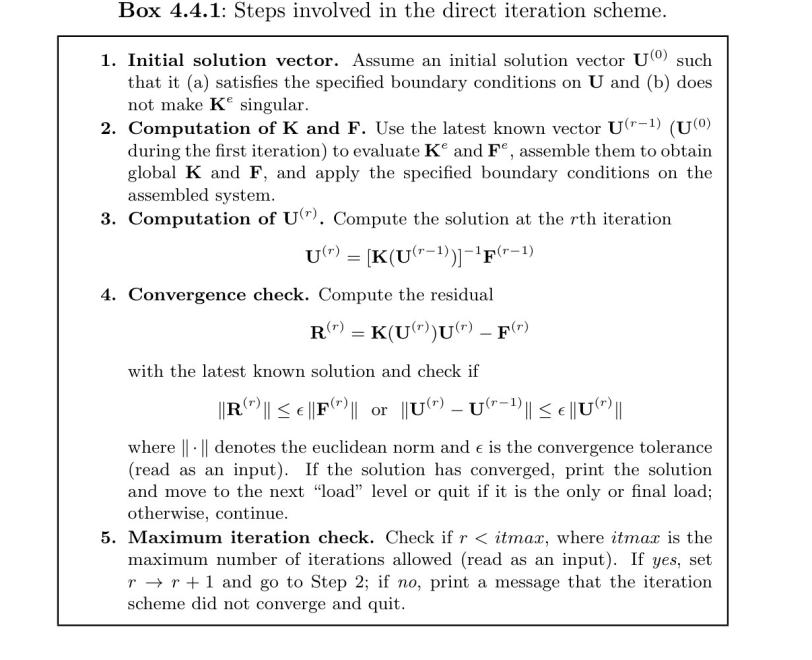
\includegraphics[width=0.8\linewidth]{\pth/nfem/fig13} 
			\end{figure}
		\end{itemize}
	\end{frame}


	\begin{frame}{Direct Iteration procedure}
		\begin{figure}
			\centering
			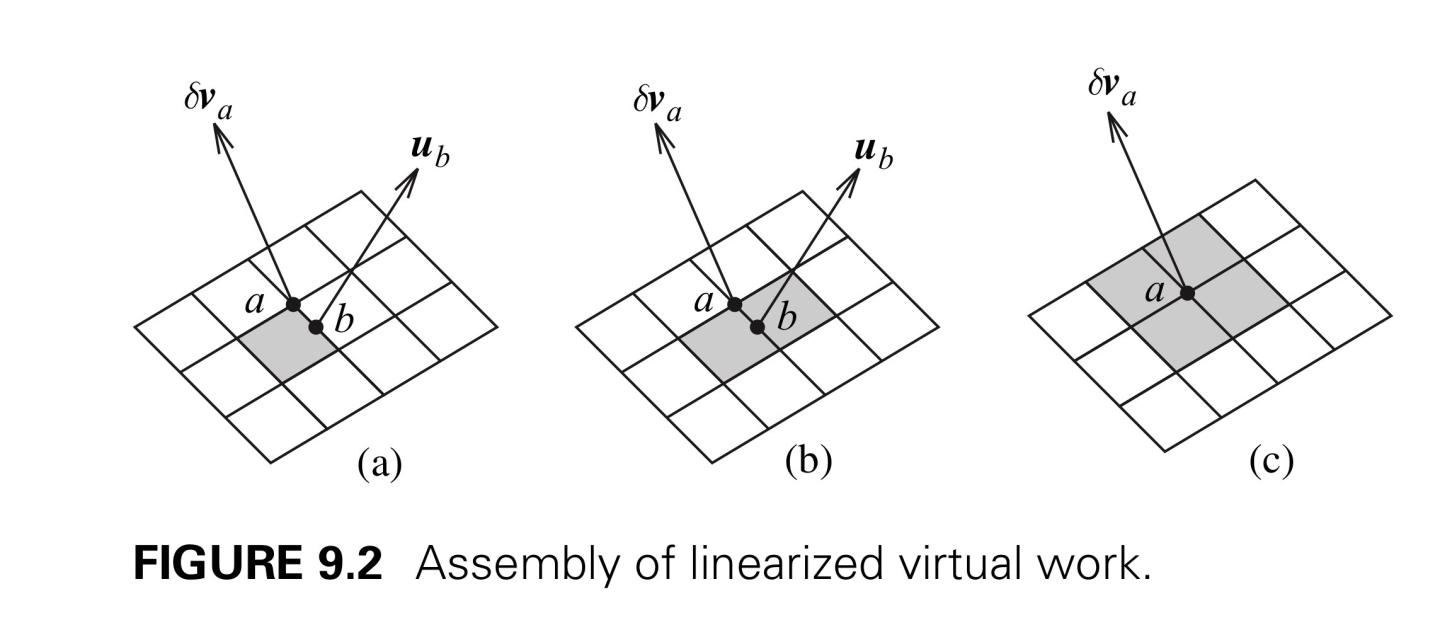
\includegraphics[width=0.5\linewidth]{\pth/nfem/fig14} 
		\end{figure}
		\begin{itemize}
			\item The method can be accelerated by using a weighted average of solutions from the last two iterations
		\begin{equation}
			\begin{aligned}
				\ve{U^r = K(\bar{U})^{-1}F(\bar{U})} \\
				\ve{\bar{U} = \beta U^{(r-2)} + (1-\beta)U^{(r-1)}}
			\end{aligned}
		\end{equation}
			\item Check Reddy 184 for some pages
		\end{itemize}
	\end{frame}


	\begin{frame}{Newtons Iteration procedure}
		\begin{itemize}
			\item In NM we expand he residual vector $\ve{R^{(r)}}$ in Taylor series about a kown solution $\ve{U^{(r-1)}}$ to get
			\begin{equation}
				\ve{R^r = R^{(r-1)} + \left(\frac{\partial R}{\partial U} \right)^{(r-1)} {\Delta} U + O(h^2)}
			\end{equation}
			where $\Delta U =  U^r - U^{(r-1)}$
			\item And saying that R in the next iteration should be zero we get
			\begin{equation}
			\begin{aligned}
				\left(\frac{\partial R}{\partial U} \right)^{(r-1)}\Delta U = -R^{(r-1)} \\
				T^{(r-1)} U^r = -R^{(r-1)}  + T^{(r-1)} U^{r-1}
			\end{aligned}
			\end{equation} 
			where T is the tangent matrix can be found at element level given as
			\begin{equation}
			\left(T_{IJ} = \frac{\partial R_I}{\partial U_J} = K_{IJ} + \sum_{m=1}^{N} \left(
			\frac{\partial K_{Im}}{\partial U_j} U_m\right) - \frac{\partial F_I}{\partial U_J} \right)^e
			\end{equation}
			The force derivative is zero if it is not a function of the load
		\end{itemize}
	\end{frame}


	\begin{frame}{NR method}
		\begin{figure}
			\centering
			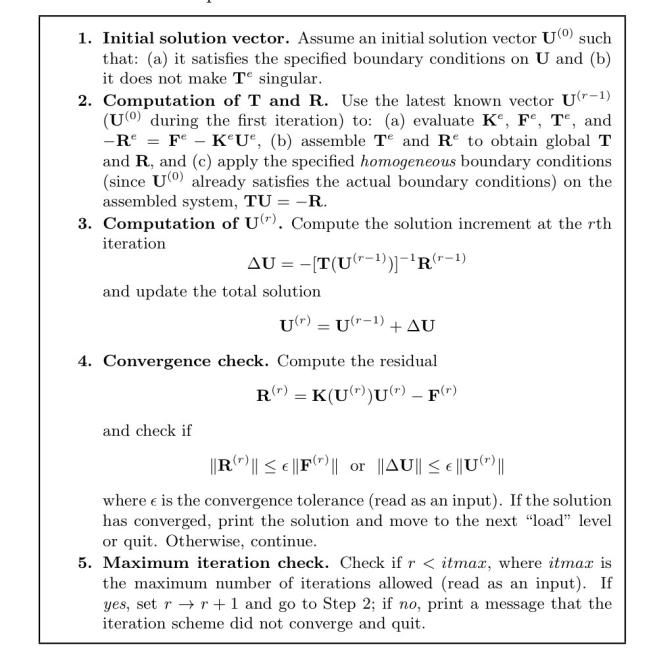
\includegraphics[width=0.5\linewidth]{\pth/nfem/fig15} 
			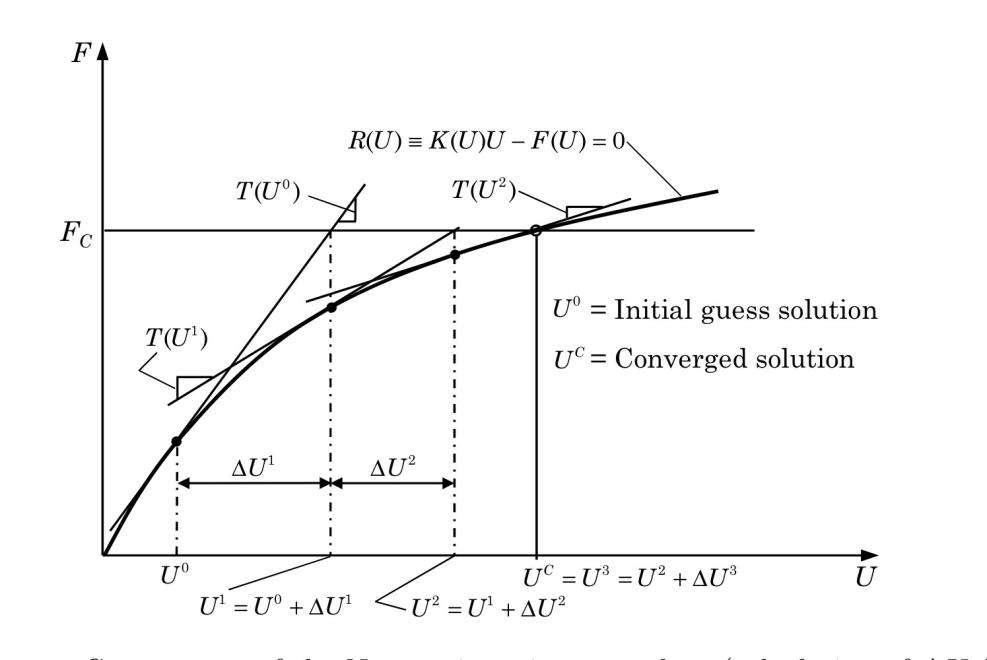
\includegraphics[width=0.45\linewidth]{\pth/nfem/fig16} 		
		\end{figure}	
	\end{frame}


	\begin{frame}{Comments}
		\begin{itemize}
			\item In the direct iteration method, the actual bc are applied at each iteration. In NR we find the increment to the known solution. If previous displ satisfies, then the increment should be zero and satisfy the boundary condition. 
			\item The symmetrry of K and T depends on the weak form. even if K is symmetric, T may not be symmetric.
			\item T can be approximate, and convergance is only when the residual is small. If it is only updated once then it is called the modified Netwons method.
			\item See the problem in Reddy -188 . Finding T	
		\end{itemize}
	\end{frame}


\section{Nonlinear Bending of straight beams}
	\begin{frame}{Introduction}
		\begin{itemize}
			\item Assuming he geomery does no change significanty, allows he principle of virtual work o be written over the underformed body. So stress is force per unit undeforemed are, strain measure of change in length w.r.t original length and shear as change in length from $\pi/2$. No distincion between Piola kirchoff and cauchy stress
			\item Nonlinearity comes solely from inplane forces proportional to he square of the rotation of a transverse normal line in the beam
			\item There are two theories
				\begin{itemize}
					\item Euler bernoulli beam (EBT)
					\item Timoshenko beam (TBT)
					
				\end{itemize}
		\end{itemize}
	\end{frame}


	\begin{frame}{Euler-Bernoulli Beam theory}
		Assumptions:
		\begin{itemize}
			\item Plane sections perpendicular to he axis of the beam remain (a) plane (b) rigid (not deform) (c) rotate such that they remain plane to the deformed axis after deformation
			\item  Assumptions amount to neglection poissons effect and transverse normal and shear strains
		\end{itemize}
	\end{frame}


	\begin{frame}{Displacements and strain fields}
		\begin{itemize}
			\item 		
			\begin{figure}
				\centering
				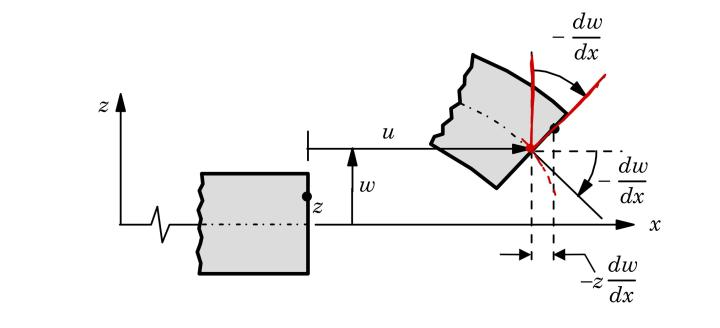
\includegraphics[width=0.7\linewidth]{\pth/nfem/fig17} 		
			\end{figure}
			The displacement is given as : $u_1 = u(x) - z\frac{d w}{d x} \qquad u_2 = 0 \qquad u_3 = w(x)$ \\
			$u_1,u_2,u_3$ is the disp of any point while $u,w$ are the disp of the centroidal axis \\
			\item So the total disp can be found from the neutral axis values. 		
			
		\end{itemize}
	\end{frame}


	\begin{frame}
		\begin{itemize}
			\item The greens theorem is
			\begin{equation}
				\begin{aligned}
					E_{ij} = \varepsilon_{ij} = \frac{1}{2}\left(\frac{\partial u_i}{\partial x_j} + \frac{\partial u_j}{\partial x_i} \right) + \frac{1}{2}\frac{\partial u_k}{\partial x_i}\frac{\partial u_k}{\partial x_j}\\
					\varepsilon_{11} = \frac{\partial u_1}{\partial x_1} + \frac{1}{2}\left[\left(\frac{\partial u_1}{\partial x_1} \right)^2 + \left(\frac{\partial u_3}{\partial x_1} \right)^2 \right]
				\end{aligned}
			\end{equation}
			\item Now the axial strains of higher orders we can igore, bu the rotation of the line perpendicular to the beam is pretty large so we have to retain it.
			\item Non-linear strains where only squares of the rotations are included are known as von Karman nonlinearity 
			\item The zero strains are $\varepsilon_{33} = \varepsilon_{13} = 0$ so only non zero strain is
			\begin{equation}
				\varepsilon_{11} = \frac{d u}{d x} - z\frac{d^2 w}{d x^2} + \frac{1}{2} \left(\frac{dw}{dx} \right)^2 
			\end{equation}
			\item  So we have two longitudinal von karman strains:
			\begin{equation}
				\varepsilon^0_{11} = \frac{d u}{d x} + \frac{1}{2} \left(\frac{dw}{dx} \right)^2  \qquad ,  \quad 
				\varepsilon^1_{11} = - z\frac{d^2 w}{d x^2} 
			\end{equation}
		\end{itemize}
	\end{frame}


	\begin{frame}{Virtual displacments : Weak form}
		\begin{itemize}
			\item The weak form can be found withou knowing the governing d.e
			\item If a body is in equilibrium, the toal virtual work done in moving through the repsective displacements is zero
			\begin{equation}
				\delta W^e = \delta W_I^e + \delta W_E^e
			\end{equation}
			$\delta W_I^e$ denotes the virtual strain stored due to the actual cauchy or second piolay stresses (Same geom) $\sigma_{ij}$\\
			$\delta W_E^e$ is the work done by external applied loads	
		\end{itemize}
	\end{frame}


	\begin{frame}
		\begin{itemize}
			\item So we have
			\begin{equation}
			\begin{aligned}
			\delta W_I^e = \int_V^e \delta \varepsilon_{xx} \sigma_{xx} dV = \int_{x_a}^{x_b} \int_A^e \left(\frac{d \delta u}{dx} + \frac{dw}{dx}\frac{d\delta w}{dx} - z \frac{d^2\delta w}{dx^2} \right) dA dx \\
			\delta W^e_E = - \left[\int_{x_a}^{x_b} q \delta w dx + \int_{x_a}^{x_b} f \delta u dx + \sum_{i=1}^{6}Q_i^e \delta \Delta_i^e \right] 
			\end{aligned}
			\end{equation}	
			\begin{figure}
				\centering
				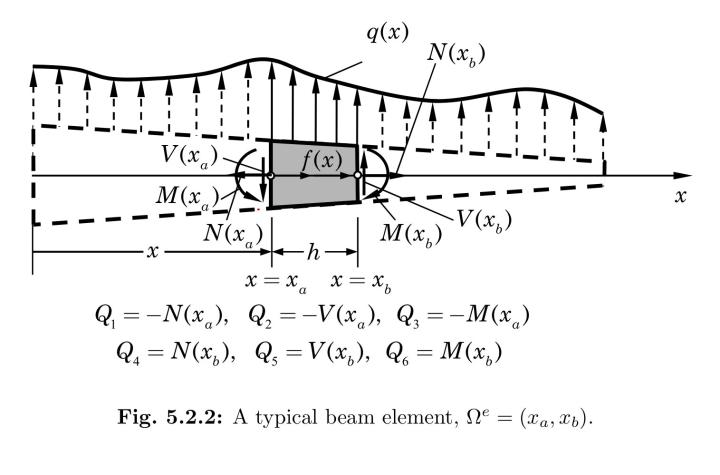
\includegraphics[width=0.7\linewidth]{\pth/nfem/fig18} 		
			\end{figure}
			
		\end{itemize}
	\end{frame}


	\begin{frame}{Sign conventions}
		\begin{figure}
			\centering
			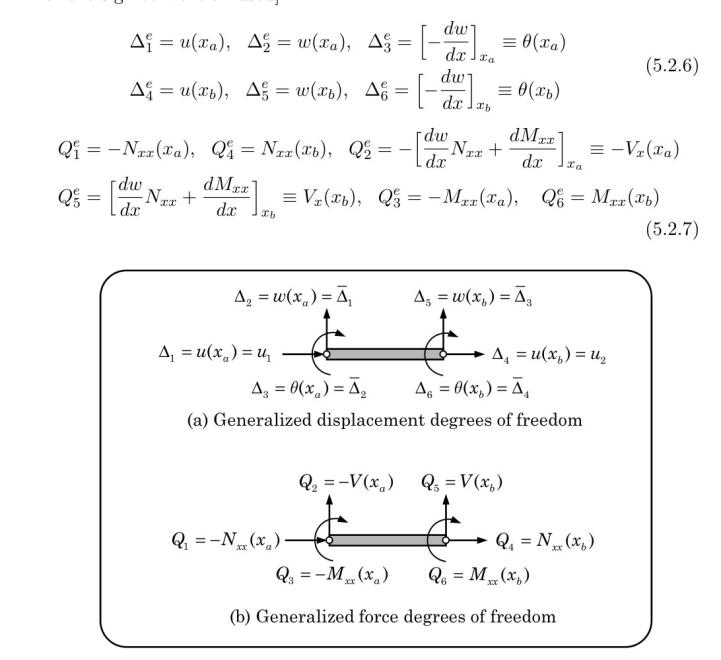
\includegraphics[width=0.6 \linewidth]{\pth/nfem/fig19} 		
		\end{figure}	
		\begin{itemize}
			\item The main thing is that for $V_x$, the component of $N_x$ is $sin(\frac{dw}{dx}) \approx \frac{dw}{dx}$, and also in moment equilibirum we get $N_{xx}\frac{dw}{dx}\Delta x = N_{xx}\Delta w$
			
		\end{itemize}
	\end{frame}


	\begin{frame}
		\begin{itemize}
			\item The free body diagram is what it is. But we can take our generalised displacement and force dof signs based on what we want.
			\item Generalised is used to show that rotationsa and moments are treated as displacements and forces
			\item By integrating in the area we get the virtual work as 
			\begin{equation}
				\delta W_I^e = \int_{x_a}^{x_b} \left[  \left(\frac{d \delta u}{dx} 
				+ \frac{dw}{dx}\frac{d\delta w}{dx} \right)N_{xx} - \frac{d^2 \delta w}{dx^2} M_{xx}\right] - \int_{x_a}^{x_b} \delta w q dx - \int_{x_a}^{x_b} \delta u f dx  - \sum_{i=1}^{6} \delta \Delta_i^e Q_i^e
			\end{equation}
			where $N_{xx} = \int_A \sigma_{xx}dA \qquad M_{xx} = \int_A \sigma_{xx}zdA$ 
		\end{itemize}
	\end{frame}


	\begin{frame}
		By taking the individual virtual terms, as the coefficients have to seperately equal to zero we get \\
		$\int_{x_a}^{x_b} \left( \frac{d\delta u}{dx}N_{xx} -\delta u f\right)dx - \delta \Delta_1^e Q_1^e - \delta \Delta_4^e Q_4^e = 0$\\
		$\int_{x_a}^{x_b} \left( \frac{d\delta w}{dx}\left(\frac{dw}{dx}N_{xx} \right) -\frac{d^2 \delta w }{dx^2}M_{xx} - \delta w q\right)dx - \delta \Delta_2^e Q_2^e - \delta \Delta_3^e Q_3^e - \delta \Delta_5^e Q_5^e -  \delta\Delta_6^e Q_6^e = 0$
		\begin{itemize}
			\item By integration by parts we get the euler lagrange equilibrium equations : given as 
			\begin{equation}
				\begin{aligned}
					\int_{x_a}^{x_b} \delta u\left( -\frac{d\delta N_{xx}}{dx} - f\right)dx - \delta \Delta_1^e Q_1^e + \left[\delta u N_{xx}\right]_{x_b}^{x_a} - \delta \Delta_4^e Q_4^e = 0\\
					\int_{x_a}^{x_b} - \delta w\left( \frac{d}{dx}\left(\frac{dw}{dx}N_{xx} \right) +\frac{d^2 M_{xx}}{dx^2} + q\right)dx - \left[ \frac{d\delta w}{dx} M_{xx}\right]_{x_b}^{x_a}  \\+  \left[ \delta w \left(\frac{dw}{dx}N_{xx} + \frac{d M_{xx}}{dx}  \right)\right]_{x_b}^{x_a} - \delta \Delta_2^e Q_2^e - \delta \Delta_3^e Q_3^e -  \delta\Delta_5^e Q_5^e -  \delta\Delta_6^e Q_6^e = 0
				\end{aligned}
			\end{equation}
		\end{itemize}
	\end{frame}


	\begin{frame}
		\begin{itemize}
			\item We get our euler equations from coefficients of the two variations
			\begin{equation}
			\begin{aligned}
				-\frac{dN_{xx}}{dx} = f(x) \\
				-\frac{d}{dx}\left(\frac{dw}{dx}N_{xx} \right) - \frac{d^2 M_{xx}}{dx^2} = q(x)
			\end{aligned}
			\end{equation}
			\item We get our boundary conditions as follows :
			\begin{equation}
			\begin{aligned}
			  Q_1^e = -N_{xx}(x_a) \qquad \qquad Q_4^e = N_{xx}(x_b) \\
			  Q_2^e = -\left[ \frac{dw}{dx}N_{xx} + \frac{dM_{xx}}{dx}\right]_{x_a} \quad 
			  Q_5^e = \left[ \frac{dw}{dx}N_{xx} + \frac{dM_{xx}}{dx}\right]_{x_b} \\
			  Q_3^e = M_{xx}(x_a) \qquad\qquad  Q_6^e = M_{xx}(x_b) \\
			\end{aligned}
			\end{equation}
			Again the - sign makes all the Qs positive in the equation
		\end{itemize}
	\end{frame}


	\begin{frame}
		\begin{itemize}
			\item We can also find the differential equations by writing the equilibirum equaitons (Fx,Fy,Mz = 0) for a small element and then take $\Delta x \rightarrow 0$. But we don't get the boundary conditions by using this. 
			\item After getting the euler lagrange differnetial equations, we can again use the weighted residual method to find the stiffness forms
			\begin{figure}
				\centering
				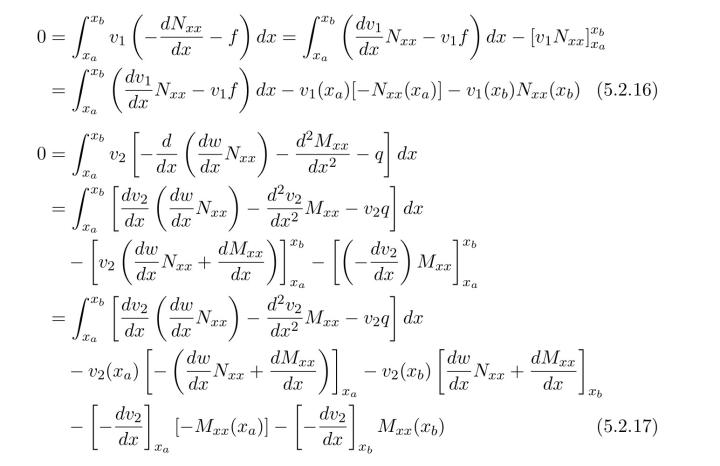
\includegraphics[width=0.8 \linewidth]{\pth/nfem/fig20} 		
			\end{figure}
			\item We clearly see that the weights are nothing but the variations and the external load work has been replaced by the internal force equivalents!!!!
		\end{itemize}
	\end{frame}


	\begin{frame}
		\begin{itemize}
			\item Now the funny thing is that we kept as N and M and now we shall replace them by 
			\begin{equation}
				\begin{aligned}
					N_{xx} = \int_A \sigma_{xx} dA = \int_{A^e} E^e \left[\frac{du}{dx} + \frac{1}{2}(\frac{dw}{dx})^2 - z\frac{d^2w}{dx^2} \right] dA \\
					= A^e \left[\frac{du}{dx} + \frac{1}{2}(\frac{dw}{dx})^2 \right] - B^e z\frac{d^2w}{dx^2}\\
					M_{xx} = \int_{A^e} \sigma_{xx} z dA = B^e  \left[\frac{du}{dx} + \frac{1}{2}(\frac{dw}{dx})^2 \right] - D^e \frac{d^2w}{dx^2}
				\end{aligned}
			\end{equation}
			where $A = EA,\qquad B = 0 \left(\int z dA = 0 \right) ,\qquad D = EI \left(\int z^2 dA \right)$
			\item Therefore the virtual work equations can be written as
			\begin{equation}
			\begin{aligned}
				0 = \int_{x_a^e}^{x_b^e} \left( A \frac{d\delta u}{x} \left[\frac{du}{dx} + \frac{1}{2}\left(\frac{dw}{dx} \right)^2 \right] -f\delta u\right) dx - \delta u(x_a)Q_1 - \delta u(x_b)Q_4 \\
				0 = \int_{x_a^e}^{x_b^e} \left( \frac{d\delta w}{dx}\frac{dw}{dx}A \left(\frac{du}{dx} + \frac{1}{2}\left(\frac{dw}{dx} \right)^2 \right) + D \frac{d^2 \delta w}{dx^2} \frac{d^2w}{dx^2} - q\delta w  \right) dx  \\ - \delta w(x_a) Q_2 - \delta \theta(x_a)Q_3 - \delta w(x_b) Q_5- \delta \theta(x_b)Q_6 
			\end{aligned}
			\end{equation}
		\end{itemize}
	\end{frame}


	\begin{frame}{FEM}
		\begin{itemize}
			\item We take the rotation as $\theta = - \frac{dw}{dx}$
			\item  We approximate the axial disp as linear lagrange and the transverse with hermite cubic interpolation functions 
		\end{itemize}
	\end{frame}


	\begin{frame}{FEM}
		\begin{figure}
			\centering
			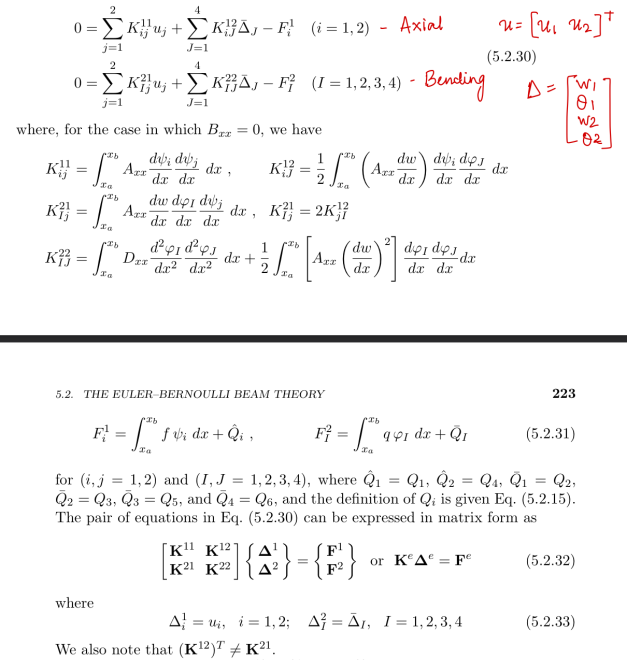
\includegraphics[width=0.66 \linewidth]{\pth/nfem/fig21} 		
		\end{figure}
	\end{frame}


	\begin{frame}
		\begin{itemize}
			\item Note that the Stiffness is not symmetric. When nonlinearity is not there then 12 and 21 (which depend on w) become 0 and the system is uncoupled. That is axial is only dependant on $u$ and bending only dependant on $\Delta$.
			\item See that we have tried to keep the shape functions symmetric
			\item When we find these conefficients from the previous iteration and then we say that the equations are linearised
			\item  The coefficients can be different if we had accounted for the terms differently, and uncouple then to a system of equations . Read reddy page 223 for this (Did not understand as of now)
			\item  We can also decompose the matrix because the 12 and 21 terms are very similar (Reddy 224)
			\item We obviously solve using direct iterative or NR method. Check reddy for the derivations of T 
		\end{itemize}
	\end{frame}


	\begin{frame}{Membrane locking}
		\small
		\begin{itemize}
			\item For the von Karman nonlinearity, for two beams : roler roler and pined pined under transverse loading. Will not have $u = 0$ because of the coupling and the solution will not be thesame. 
			\item  Suppose the roler roler beam has a constraint on u in the middle to remove rigid body movemenl, and transverse load does not make axial strain because the beam can slide without making stresses. This will have higher transverse deflection because it can stretch.
			\item The pined pined however has constraints on x = 0 and x = L so it will develop axial strains.
			\item  To make sure that the roler roler does not have any axial strain \\
			$\varepsilon_{xx}^o = \frac{du}{dx}+\frac{1}{2}(\frac{dw}{dx})^2 = 0$\\
			And basically both shoud be of the same order $-\frac{du}{dx} = \left(\frac{dw}{dx} \right)^2$
			\item So when w is cubic $\frac{dw}{dx}$ is square and the power makes it quad. So $u$ should be atleast order fifth. Taking u with any polynomial less , will make the constraint not satisfied and stiff, giving zero displacement field. (Membrane locking)
			\item We can also treat the axial strain  as constant. Since $\frac{du}{dx}$ is const, we can make $(\frac{dw}{dx})^2$ also constant. We can do this by reduced integration of all nonlinear stiffness coefficients (A,B,D).
		\end{itemize}
	\end{frame}


	\begin{frame}{Computation of stresses and strains}
		\begin{itemize}
			\item Strains and stresses are close when found at the Gauss points
			\item u is aprrox with linear lagrange and w is approx with hermite cubic polynomials.
			\item Membrane strain $\varepsilon^0_{xx}$ is assumed constant is evaluated using one point G.Q, and the bending strain $\varepsilon^1_{xx}$ is also linear and done by one point G.Q.
			\item 
			\begin{equation}
			\begin{aligned}
				\varepsilon^0_{xx} = \frac{du}{dx} + \frac{1}{2}\left(\frac{dw}{dx} \right)^w \\ 
				\varepsilon^1_{xx} = -\frac{d^2w}{dx^2}
			\end{aligned}
			\end{equation}
			And the stresses are given as follows :
			\item $\sigma_{xx} = \sigma_{xx}^0 + z\sigma_{xx}^1 = E \varepsilon_{xx}^0 + z E \varepsilon_{xx}^1$ \\
			
		\end{itemize}
	\end{frame}



	\begin{frame}{Timoshenko beam theory (TBT)}
		\begin{itemize}
			\item The euler bernoulli beam is based on fact that a straight line transverse to axis before defomration remains (1) straight (2) inextensible (3) normal to mid plane after deformation. In TBT, we say the last assumption, the rotation is independant of the slope
			\item So we get the displacement field with an independant slope
			\begin{equation}
				u_1 = u(x) + z \phi_x(x) \qquad u2 = 0 \qquad u_3 = w(x)
			\end{equation} 
			\item The non zero strains are :
			\begin{equation}
			\begin{aligned}
				\varepsilon_{xx} = \frac{du_1}{dx} + \frac{1}{2}(\frac{du_3}{dx})^2 = \frac{du}{dx} + \frac{1}{2}(\frac{dw}{dx})^2 + z \frac{d\phi}{dx} = \varepsilon^0_{xx} + z\varepsilon^1_{xx} \\
				\gamma_{xz} = \frac{du_1}{dz}  \frac{du_3}{dx} = \phi + - \left(-\frac{dw}{dx} \right) = \gamma_{xz}^0
			\end{aligned}
			\end{equation}	
			The last one we get because we remove the rotation due to w
		\end{itemize}
	\end{frame}


	\begin{frame}
		\begin{itemize}
			\item The virtual strains are :
			\begin{equation}
				\begin{aligned}
					\delta \varepsilon_{xx}^0 = \frac{d\delta u}{dx} + \frac{dw}{dx}\frac{d\delta w}{dx} \\
					\delta \varepsilon^1_{xx} = z \frac{d\phi}{dx} \\
					\delta \gamma_{xz} = \delta \phi + \frac{d \delta w}{dx} 
				\end{aligned}
			\end{equation}	
		\end{itemize}
		\begin{figure}
			\centering
			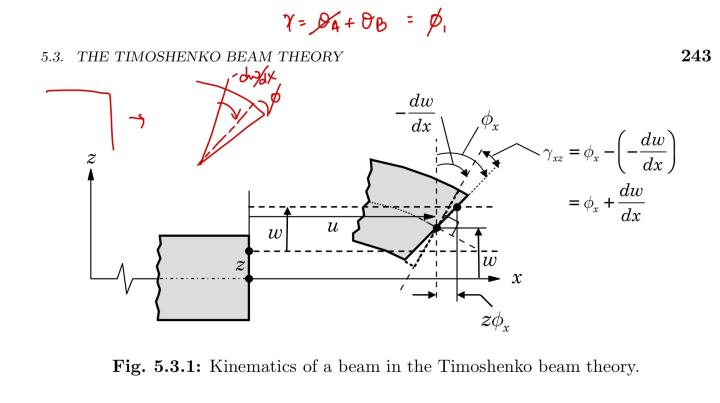
\includegraphics[width=0.66 \linewidth]{\pth/nfem/fig22} 		
		\end{figure}
	\end{frame}


	\begin{frame}{Weak form}
		\begin{itemize}
			\item The weak form is similaly developed (Reddy 243)
			\begin{equation}
			 \delta W = \int_{x_a^e}^{x_b^e} \int_{A^e} \left(N_{xx} \delta \varepsilon_{xx}^0 + M_{xx}\delta\varepsilon_{xx}^1 + Q_x \delta\varepsilon_{xz}^0 \right) - \delta W_E^e
			\end{equation}
			Note that : \\
			$N = \int \sigma dA, \quad M =  \int \sigma z dA \quad Q =  \int \sigma_{xz}dA$ \\
			$\sigma =  E\varepsilon \quad \sigma_{xz} = KG\gamma_{xz}$
			\\
			The K thing is cause we assume a constant shear over the cross section when we just say stress is G x strain. So it is a correcting factor! We compare the two energies and then we find K.
			\item Trying to keep all the variations in the same derivative order, we get the euler equilibrium equations, taking each coefficient as zero
			\begin{equation}
				\begin{aligned}
					\delta u : \quad -\frac{dN}{dx} = f(x) \\
					\delta w : \quad -\frac{dQ}{dx}  - \frac{d}{dx}\left(N \frac{dw}{dx} \right) = q(x)\\
					\delta\phi : -\frac{dM}{dx} + Q_x = 0
				\end{aligned}
			\end{equation}
			u,w, $\phi$ are the primary and N,Q,M are the secondary variables
		\end{itemize}
	\end{frame}


	\begin{frame}
		\begin{itemize}
			\item We keep the secondary variables in terms of the independant primary variables
			\begin{equation}
			\begin{aligned}
				N = A \left[ \frac{du}{dx} + \frac{1}{2} \left(\frac{dw}{dx} \right)^2\right] + B \frac{d\phi}{dx} \\
				M = B \left[ \frac{du}{dx} + \frac{1}{2} \left(\frac{dw}{dx} \right)^2\right] + D \frac{d\phi}{dx} \\
				Q = S \left(\frac{dw}{dx} + \phi \right)
			\end{aligned}
			\end{equation}
			 A,B,D are the previous terms moments of area giving the integral only in the x direction in the virtual work. S is the shear stiffness given as $S = K \int G dA = K G A =  \frac{KEA}{2(1+ \nu)}$
			 \item  Obviously we can derive the governing differential equilibrium equations (Page 245). For homogeneous beams , we have B = 0. which are the equilibrium equations given by the variational principle
		\end{itemize}
	\end{frame}


	\begin{frame}{FEM}
		\begin{itemize}
			\item The virtual work statement is then given as 
			\begin{figure}
				\centering
				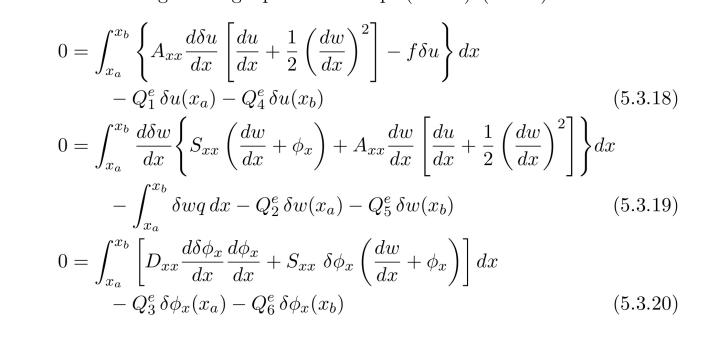
\includegraphics[width=0.8 \linewidth]{\pth/nfem/fig23} 		
			\end{figure}
			\item  The Q's have the same meaning as the euler bernoulli element
		\end{itemize}
	\end{frame}


	\begin{frame}{FEM}
		\begin{figure}
			\centering
			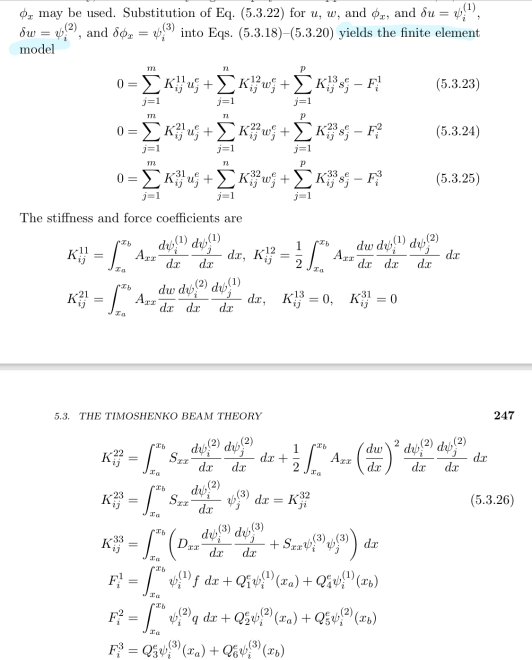
\includegraphics[width=0.5 \linewidth]{\pth/nfem/fig24} 		
		\end{figure}
		\begin{itemize}
			\item We then get $\ve{Ku = F}$ where $\ve{u = \mat{u,w,\phi}^T}$. Check Reddy 249 for T stiffness derivation
			
		\end{itemize}
	\end{frame}


	\begin{frame}{Shear and Membrane locking}
		\begin{itemize}
			\item Timoshenko beam without von Karman nonlinearity differ from each other in the choice of the approx function for w and $\phi$. Some are equal and others different
			\item Linear interpolation of both w and $\phi$ is the easisest. This makes the slope $\frac{dw}{dx}$ constant. In a think beam, as the length to thickness ratio becomes large (100), the slope would be equal to $-\phi$ which is linear instead of constant. 
			\item On the other hand a constant $\phi$ leads to zero bending energy while the transverse shear is nonzero. 
			\item  Check Reddy 248 ( Have not understood fully Locking issue)
			\item The primary variables may not be approximated by the same shape functions :
			\begin{equation}
			u(x) = N^1_iu_i \qquad w(x) = N^2_iw_i \qquad \phi(x) = N^3_i\phi_i
			\end{equation}
		\end{itemize}
	\end{frame}


	\begin{frame}{Functionally graded materials}
		Check reddy
	\end{frame}
	
	
	
	\section{Two dimensional problems having a single variable}
	\begin{frame}{Model equation}
		\begin{itemize}
			\item Suppose we are trying to find the solution $u(x,y)$ of the following partial differential equation
			\begin{equation}
			 -\frac{d}{dx}\left(a_{xx} \frac{\partial du}{\partial dx} + a_{xy} \frac{\partial u}{\partial y} \right)
			 -\frac{d}{dy}\left(a_{yx} \frac{\partial du}{\partial dx} + a_{yy} \frac{\partial u}{\partial y} \right) + a_{00} u = f(x,y) \quad \text{in} \quad \Omega
			\end{equation}	
			The coefficients are also a function o u : eg $a_{xx} = f(x,y,u,\frac{\partial u}{\partial x }, \frac{\partial u}{\partial y})$
			\item When we descritize it with $\bar{\Omega}$ with a boundary $\bar{\Gamma}$, we get a residual given as :
			\begin{equation}
				R(u_h) = 
				-\frac{d}{dx}\left(a_{xx} \frac{\partial du_h}{\partial dx} + a_{xy} \frac{\partial u_h}{\partial y} \right)
				-\frac{d}{dy}\left(a_{yx} \frac{\partial du_h}{\partial dx} + a_{yy} \frac{\partial u_h}{\partial y} \right) + a_{00} u = f(x,y)
			\end{equation}
		\end{itemize}
	\end{frame}


	\begin{frame}{Weak form}
		The step is to multiply the residual with the ith weight function $w_i(x,y)$ which should be differentiable too. We then set $w_iR$ over the element domain $\Omega^e = 0$
		\begin{itemize}
			\item $0 = \int_{\Omega_e} w_i \left[ 
			-\frac{d}{dx}\left(a_{xx} \frac{\partial u_h}{\partial x} + a_{xy} \frac{\partial u_h}{\partial y} \right)
			-\frac{d}{dy}\left(a_{yx} \frac{\partial u_h}{\partial x} + a_{yy} \frac{\partial u_h}{\partial y} \right) + a_{00} u - f(x,y) \right] dxdy$
			\item Now we know : $\frac{d}{dx}\left(w \frac{du}{dx}\right) = w\frac{d^2u}{dx^2} + \frac{dw}{dx}\frac{du}{dx}$ \\ and $\int_A \frac{d}{dx}\left(w \frac{du}{dx} \right) dA= \int_S \left(w \frac{du}{dx} \right) dS$
			\item We get 
			\begin{equation}
			\begin{aligned}
			0 = \int_A \left[\frac{\partial w_i}{\partial x} \left(a_{xx} \frac{\partial u_h}{\partial x } + a_{xy} \frac{\partial u_h}{\partial y }\right) + 
			\int_A \frac{\partial w_i}{\partial y} \left(a_{yx} \frac{\partial u_h}{\partial x } + a_{yy} \frac{\partial u_h}{\partial y }\right) + a_{00}w_iu_h - w_if \right]dxdy \\
			- \int_S w_i \left[ \left(a_{xx} \frac{\partial u_h}{\partial x} + a_{xy} \frac{\partial u_h}{\partial y} \right)n_x + \left(a_{yx} \frac{\partial u_h}{\partial x} + a_{yy} \frac{\partial u_h}{\partial y} \right)n_y \right]dS
			\end{aligned}
			\end{equation}
			where $\ve{n = n_xe_1 + n_ye_2}$ which gives the direction consies of the boundary $\Gamma^e$. The second term can also be written as $-\int_S q_n dS$ which is the external flux normal as we move counter clockwise. 
		\end{itemize}
	\end{frame}


	\begin{frame}
		\begin{figure}
			\centering
			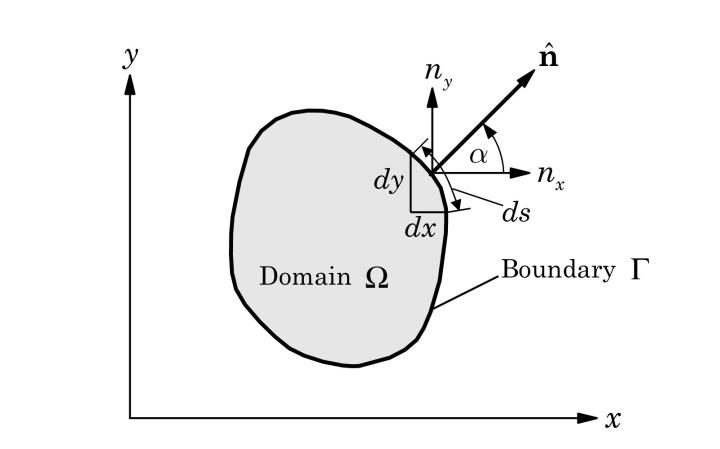
\includegraphics[width=0.5 \linewidth]{\pth/nfem/fig25} 		
		\end{figure}
	\begin{itemize}
		\item In the case of heat transfer through an anisotropic medium, aij denotes the conductivity and qn is the normal heat flux
		
	\end{itemize}
	\end{frame}


	\begin{frame}{FEM}
		\begin{itemize}
			\item The weak form states that u should be atleast linear in both x and y
			\item $u_h^e = \sum u_iN_i(x,y)$ with $N_i(x_j,y_j) = \delta_{ij} $ and $\sum_j N_j(x,y)=1$
			\begin{figure}
				\centering
				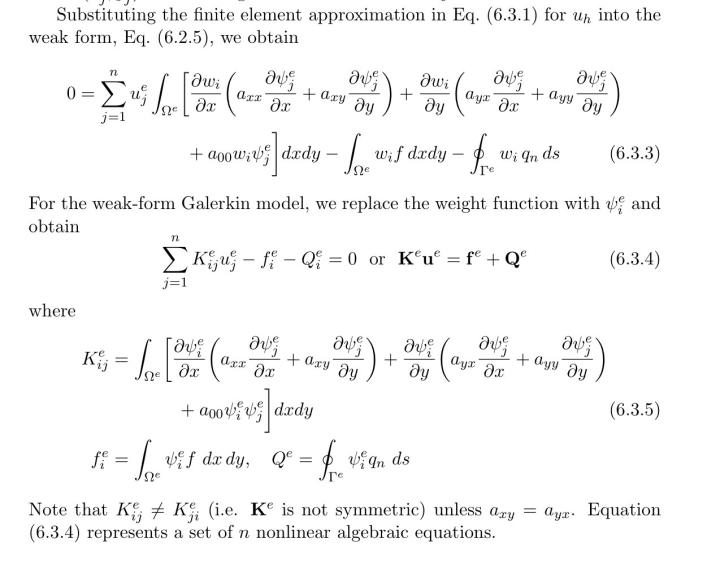
\includegraphics[width=0.8 \linewidth]{\pth/nfem/fig26} 		
			\end{figure}	
		\end{itemize}
	\end{frame}


	\begin{frame}
		\begin{itemize}
			\item The equations have to be solved by nonlinear methods
			\item The tangent T is given in page 271
		\end{itemize}
	\end{frame}


	\begin{frame}{Axisymmetric problems}
		\begin{itemize}
			\item The differential equation in cylindrical coordinate system (r,$\theta,z$)
			\begin{equation}
				-\frac{1}{r}\frac{\partial}{\partial r}\left(ra_{rr}\frac{\partial u}{\partial r} \right)
				- \frac{1}{r^2}\frac{\partial}{\partial \theta}\left(a_{\theta\theta}\frac{\partial u}{\partial \theta} \right)
				- \frac{\partial}{\partial z}\left(a_{zz}\frac{\partial u}{\partial z} \right) = f
			\end{equation} 
			\item where u,f and the coefficients are a function of (r,$\theta,z$)
			\item Dependant on the coefficents, boundary conditions and load f the problem can be made to 2D or even 1D
			\item If the cylinder is very long and stuff dont vary and depend on z, then we can assume a disk. No also if there is independance from $\theta$ then we can even just do a radial line \footnote{We just remove the derivatives in the equations where the change will be zero}
			\begin{figure}
				\centering
				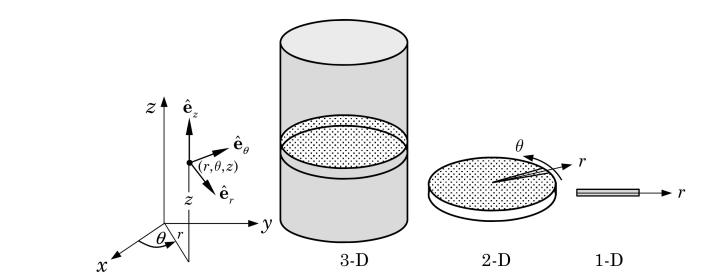
\includegraphics[width=0.8 \linewidth]{\pth/nfem/fig27} 		
			\end{figure}
		\end{itemize}
	\end{frame}


	\begin{frame}{FEM}
		\begin{itemize}
			\item Suppose all the variables are not dependant on $\theta$, therefore we would get something like a plane and the Governing differential equation will be
			\begin{equation}
				-\frac{1}{r}\frac{\partial}{\partial r}\left(ra_{rr}\frac{\partial u}{\partial r} \right)
				- \frac{\partial}{\partial z}\left(a_{zz}\frac{\partial u}{\partial z} \right) = f(r,z)
			\end{equation}
			\item The weighted statement and weak form (Using greens theorem) will be given as :
			\begin{equation}
			\begin{aligned}
			 0 = \int_A w_i \left[ 	-\frac{1}{r}\frac{\partial}{\partial r}\left(ra_{rr}\frac{\partial u}{\partial r} \right)
			 - \frac{\partial}{\partial z}\left(a_{zz}\frac{\partial u}{\partial z} \right) - f(r,z)\right] rdrdz \\
			 = \int_A \left[ a_{rr}(r,z,u_h) \frac{\partial w_i}{\partial r}\frac{\partial u_h}{\partial r}
			 + a_{zz}(r,z,u_h) \frac{\partial w_i}{\partial z} \frac{\partial u_h}{\partial z}\right] rdrdz - \int_A w_if(r,z)rdrdz - \int_S w_iq_n ds 
			\end{aligned}
			\end{equation}
			where $q_n = r\left[ a_{rr} \frac{\partial u_h}{\partial r}n_r + a_{zz}\frac{\partial u_h}{\partial z} n_z\right]$
			\item And we get $\ve{Ku = f+Q = F}$
			\item Remember the shape functions are functions of N(r,z)	
	\end{itemize}
	\end{frame}


	\begin{frame}{Numerical integration}
		\begin{itemize}
			\item
			\begin{figure}
				\centering
				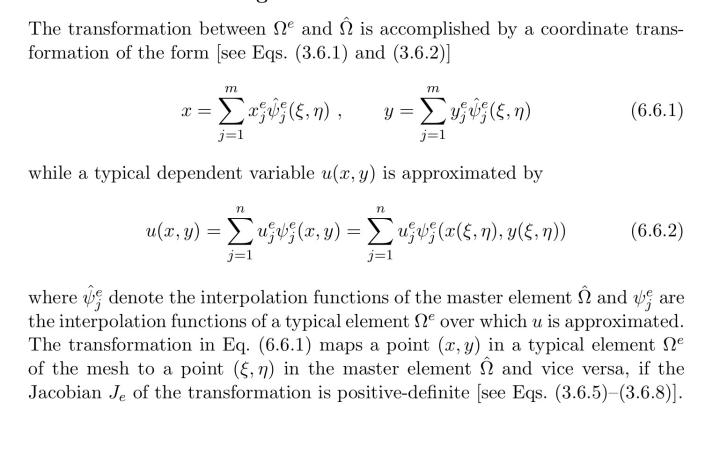
\includegraphics[width=0.9 \linewidth]{\pth/nfem/fig28} 		
			\end{figure} 
			
		\end{itemize}
	\end{frame}

	
	\begin{frame}{Gauss quad - coordinate change}
		\begin{itemize}
			\item Remember that we have to we have to transform the integral domain to the master element so that Gauss quadrature can be usd. The derivatives in the original geometry are also expressed with respect to $\xi,\eta$ given by
			\begin{equation}
			\mat{\frac{\partial N_i}{\partial dx}; ;\frac{\partial N_i}{\partial dy} } = \ve{J^{-1}} \mat{\frac{\partial N_i}{\partial d\xi}; ;\frac{\partial N_i}{\partial d\eta} } 
			\end{equation}
			where $\ve{J} = \mat{\frac{\partial x}{\partial \xi}, \frac{\partial y}{\partial \xi}; , ; \frac{\partial x}{\partial \eta}, \frac{\partial y}{\partial \eta}} =
			\mat {\sum x_i \frac{\partial N_i}{\partial \xi}, \sum y_i \frac{\partial N_i}{\partial \xi} ; , ; 
			\sum x_i \frac{\partial N_i}{\partial \eta}, \sum y_i \frac{\partial N_i}{\partial \eta}} = \mat{\frac{\partial N_1}{\partial \xi}, \frac{\partial N_2}{\partial \xi}, .... ,\frac{\partial N_m}{\partial \xi} ; , , ,;
			\frac{\partial N_1}{\partial \eta}, \frac{\partial N_2}{\partial \eta}, ...., \frac{\partial N_m}{\partial \eta} }
	 		\mat{x_1, y_1; , ; x_2, y_2; , ; \vdots, \vdots; x_m,y_m}$ 
	 		\item If the same shape functionsa re used for the geometry and field variable, we say its isoparametric
		\end{itemize}
	\end{frame}


	\begin{frame}
		\begin{figure}
			\centering
			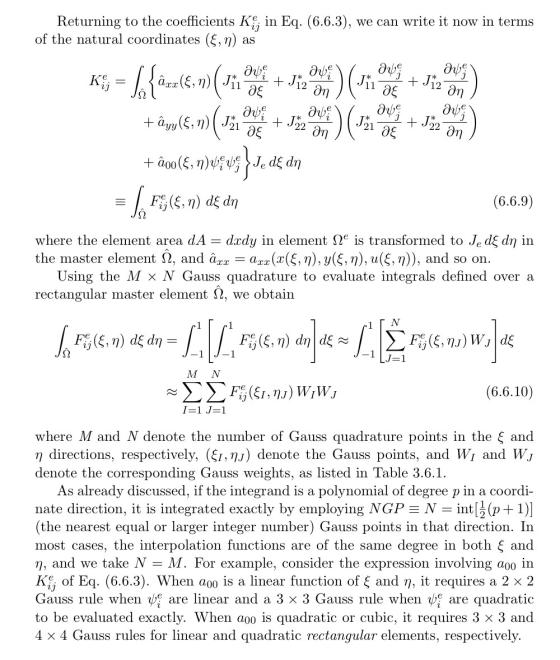
\includegraphics[width=0.6 \linewidth]{\pth/nfem/fig29} 		
		\end{figure} 
	where J* are the components of the inverse jacobian
	\end{frame}


	\section{Time dependant problems}
	
	\begin{frame}{Time dependacy}
		Will have to read later!!
	\end{frame}



\section{Plates}

	\begin{frame}
		\begin{itemize}
			\item Plate has large dimension compared to thickness. No need to use 3D, with study the deformations and stresses in plates, smal rotations and large displacement (w/h>1)
			\item Extension of Euler berunoulli is called Kirchoff plate. Extension of timoshenko beam is the first order or mindlin shear deformation plate theory.
			\item $\ve{X}$ is used for the material coordinates and $\ve{x}$ is used for the spatial coordinates. No distinction is made between the material and spatial coordinates. 	
		\end{itemize}
	\end{frame}


	\begin{frame}{Classical plate theory}
		The disp satisfy the kirchoff rules which are an extension of the euler bernoulli hypothesis which are
		\begin{itemize}
			\item Straight lines perpendicular to the mid surface remain straight
			\item Transverse normals do not have elongation
			\item Cross sections remain perpendiuclar under rotation
		\end{itemize}
	\end{frame}


	\begin{frame}{Dislacement and strain fields}
		\begin{itemize}
			\item We have the domain of the plate as $\Omega_o \times (-h/2,h/2)$. The boundary of the top surface $z = h/2$ and bottom surface $z = -h/2$ with boundary $\Gamma$ which is a curved surface with outward normal $\ve{n} = n_xe_1 + n_ye_2$
			\begin{figure}
				\centering
				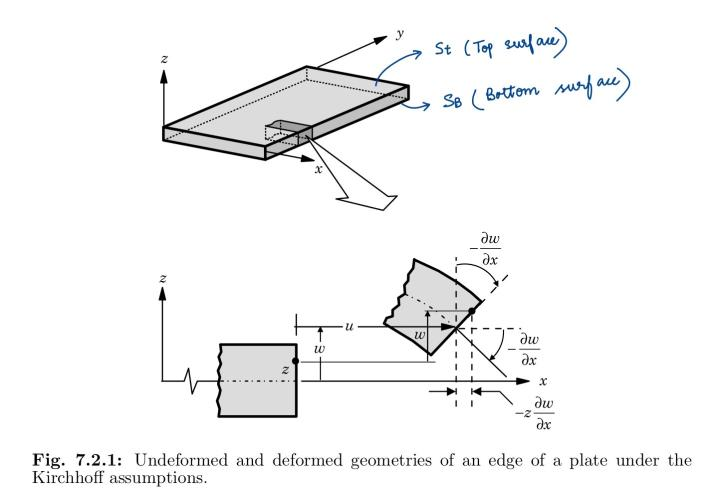
\includegraphics[width=0.8 \linewidth]{\pth/nfem/fig30} 		
			\end{figure}
		\end{itemize}
	\end{frame}


	\begin{frame}
		\begin{itemize}
			\item The kirchoff hypotehesis implies the following displacement field 
			\begin{equation}
			\begin{aligned}
				u_1(x,y,z,t) = u(x,y,t) - z\frac{\partial w}{\partial x} \\
				u_2(x,y,z,t) = v(x,y,t) - z\frac{\partial w}{\partial y} \\
				u_3(x,y,z,t) = w(x,y,t) 
			\end{aligned}
			\end{equation}
			\item Where $u,v,w$ denote the material point in the undeformed of the nerutral axis wherees $u_1,u_2,u_3$ denote any aribitary point location
			\item The componenets of the Green-Lagrange strain tensor $\ve{E}$ in terms of components of the total displacement vector $u = x(x,t) - X$ (x and X here are the same) is
			\begin{equation}
				\tiny
				\begin{aligned}
					E_{11} = \frac{\partial u_1}{\partial X_1} + \frac{1}{2}\left[ \left(\frac{\partial u_1}{\partial X_1} \right)^2 +
					\left(\frac{\partial u_2}{\partial X_1} \right)^2 + 
					\left(\frac{\partial u_3}{\partial X_1} \right)^2 \right] \\ 
					E_{22} = \frac{\partial u_2}{\partial X_2} + \frac{1}{2}\left[ \left(\frac{\partial u_1}{\partial X_2} \right)^2 +
					\left(\frac{\partial u_2}{\partial X_2} \right)^2 + 
					\left(\frac{\partial u_3}{\partial X_2} \right)^2 \right]\\
					E_{33} = \frac{\partial u_3}{\partial X_3} + \frac{1}{2}\left[ \left(\frac{\partial u_1}{\partial X_3} \right)^2 +
					\left(\frac{\partial u_2}{\partial X_3} \right)^2 + 
					\left(\frac{\partial u_3}{\partial X_3} \right)^2 \right]\\
					E_{12} = \frac{1}{2}\left[ \frac{\partial u_1}{\partial X_2} + \frac{\partial u_2}{\partial X_1} + 
					\frac{\partial u_1}{\partial X_1}\frac{\partial u_1}{\partial X_2} +
					\frac{\partial u_2}{\partial X_1}\frac{\partial u_2}{\partial X_2} +
					\frac{\partial u_3}{\partial X_1}\frac{\partial u_3}{\partial X_2} +
					\right]	\\
					E_{13} = \frac{1}{2}\left[ \frac{\partial u_1}{\partial X_3} + \frac{\partial u_3}{\partial X_1} + 
					\frac{\partial u_1}{\partial X_1}\frac{\partial u_1}{\partial X_3} +
					\frac{\partial u_2}{\partial X_1}\frac{\partial u_2}{\partial X_3} +
					\frac{\partial u_3}{\partial X_1}\frac{\partial u_3}{\partial X_3} +
					\right]	\\
					E_{23} = \frac{1}{2}\left[ \frac{\partial u_2}{\partial X_3} + \frac{\partial u_3}{\partial X_2} + 
					\frac{\partial u_1}{\partial X_2}\frac{\partial u_1}{\partial X_3} +
					\frac{\partial u_2}{\partial X_2}\frac{\partial u_2}{\partial X_3} +
					\frac{\partial u_3}{\partial X_2}\frac{\partial u_3}{\partial X_3} +
					\right]	
				\end{aligned}
			\end{equation}
		\end{itemize}
	\end{frame}


	\begin{frame}
		\begin{itemize}
			\item If the components of the displacement gradient are very small = O($\epsilon$), then the terms having O($\epsilon^2$) can be omitted in the strains. However if the rotations of the transverse normals are moderate (10 -15 degrees), then the following strains are small but not negligible
			\begin{equation}
			\left(\frac{\partial u_3}{\partial X_1} \right)^2 \qquad
			\left(\frac{\partial u_3}{\partial X_2} \right)^2 \qquad
			\frac{\partial u_3}{\partial X_1}\frac{\partial u_3}{\partial X_2}  
			\end{equation}
			\item  Thus the strains take the following (Remember that $E = \varepsilon$ where we say its small strain but moderate rotations)
			\begin{equation}
			\tiny
			\begin{aligned}
			E_{11} = \varepsilon_{11}= \frac{\partial u_1}{\partial x} + \frac{1}{2}\left[ \left(\frac{\partial u_3}{\partial x} \right)^2 \right] \qquad
			E_{22} = \frac{\partial u_2}{\partial y} + \frac{1}{2}\left[ 
			\left(\frac{\partial u_3}{\partial y} \right)^2 \right]\\
			E_{33} = \frac{\partial u_3}{\partial z} \qquad
			E_{12} = \frac{1}{2}\left[ \frac{\partial u_1}{\partial y} + \frac{\partial u_2}{\partial x} + 
			\frac{\partial u_3}{\partial x}\frac{\partial u_3}{\partial y} 
			\right]	\\
			E_{13} = \frac{1}{2}\left[ \frac{\partial u_1}{\partial z} + \frac{\partial u_3}{\partial x} 
			\right]	\qquad
			E_{23} = \frac{1}{2}\left[ \frac{\partial u_2}{\partial z} + \frac{\partial u_3}{\partial y}
			\right]	
			\end{aligned}
			\end{equation}
		\end{itemize}
	\end{frame}


	\begin{frame}
		\begin{itemize}
			\item  For this displacement field, we have $\varepsilon_{z} = \frac{\partial u_3}{\partial z} = \frac{\partial w}{\partial z} = 0$ and taking the displacement fields. The strains then reduce to
			\begin{equation}
				\begin{aligned}
				\varepsilon_{xx}= \frac{\partial u}{\partial x} + \frac{1}{2}\left[ \left(\frac{\partial w}{\partial x} \right)^2 - z \frac{\partial^2 w}{\partial x^2}\right] \qquad
				\varepsilon_{yy} = \frac{\partial v}{\partial y} + \frac{1}{2}\left[ 
				\left(\frac{\partial w}{\partial y} \right)^2 - z\frac{\partial^2 w}{\partial y^2}\right]\\
				2\varepsilon_{xy} = \gamma_{xy} = \frac{\partial u}{\partial y} + \frac{\partial v}{\partial x} + 
				\frac{\partial w}{\partial x}\frac{\partial w}{\partial y} -2z\frac{\partial^2 w}{\partial x \partial y}	\\
				2\varepsilon_{xz} = -  \frac{\partial w}{\partial x} + \frac{\partial w}{\partial x} = 0\qquad
				2\varepsilon_{yz} = - \frac{\partial w}{\partial y} + \frac{\partial w}{\partial y} = 0
				\end{aligned}
			\end{equation}
			\item These are called von Karman strains and called classical plate theory with von karman strains. Note that the transverse strains are zero in the classical plate theory. The total strains can be written as membrane + bending strain
			\begin{equation}
			\mat{\varepsilon_{xx};\varepsilon_{yy};\gamma_{xy}} =  \mat{\varepsilon_{xx}^0;\varepsilon_{yy}^0;\gamma_{xy}^0} + z\mat{\varepsilon_{xx}^1;\varepsilon_{yy}^1;\gamma_{xy}^1}
			\end{equation}
		\end{itemize}
	\end{frame}


	\begin{frame}
		\begin{itemize}
			\item The strains are expanded as : 
			\begin{equation}
			\begin{aligned}
			\mat{\varepsilon_{xx}^0;\varepsilon_{yy}^0;\gamma_{xy}^0} = 
			\mat{\frac{\partial u}{\partial x} + \frac{1}{2} \left(\frac{\partial w}{\partial x} \right)^2 ; ;
				 \frac{\partial v}{\partial y} + \frac{1}{2}\left(\frac{\partial w}{\partial y} \right)^2; ;
				\frac{\partial u}{\partial y} + \frac{\partial v}{\partial x} + 
				\frac{\partial w}{\partial x}\frac{\partial w}{\partial y} }\qquad
			\mat{\varepsilon_{xx}^1;\varepsilon_{yy}^1;\gamma_{xy}^1} = - \mat{
			\frac{\partial^2 w}{\partial x^2};; \frac{\partial^2 w}{\partial y^2};; 2\frac{\partial^2 w}{\partial x \partial y}	}
			\end{aligned}
			\end{equation}
		\end{itemize}
	\end{frame}


	\begin{frame}{Weak form of classical plate theory}
		\begin{itemize}
			\item Virtual work statement is used again to derive (Just like 4 beams). We account for thermal effects, where the material does not change with tempearture which is knowon as a fuction of the position  hence ($\delta T = 0$), so temperature eneters throught the constitutive relations.
			\item Suppose the domain is represented by fem $\Omega_e$ with  distributed transverse loads $q(x,y)$ at the top. $(\sigma_{nn},\sigma_{ns},\sigma_{nz})$ are the stress components on the boundary of the plate
			\begin{figure}
				\centering
				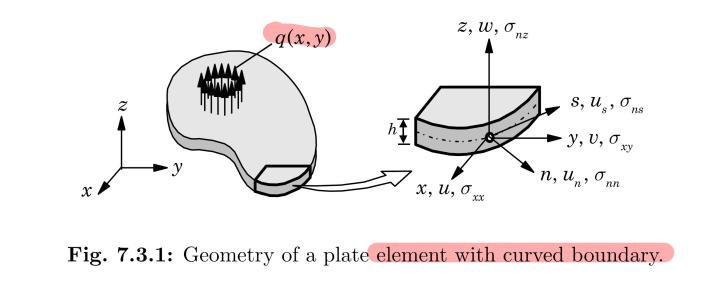
\includegraphics[width=0.8 \linewidth]{\pth/nfem/fig31} 		
			\end{figure}
		\end{itemize}
	\end{frame}


	\begin{frame}
		\begin{itemize}
			\item The principle of virtual work states that $0 = \delta W^e = \delta W_I^e + \delta W_E^e$
			\item As noted earlier, the transverse shears $\gamma_{xz},\gamma_{yz},\varepsilon_{zz}$ are zero. Therefore the transverse stresses ($\sigma_{xz},\sigma_{yz},\sigma_{zz}$ ) do not eneter the formulatin because the strains due to these are zero. Even though they are not accounted, in reality they exist to maintain equilibirum, these components can also be specified at the boudary. So they have to be accounted in the equilibirum equations. 
			\item The internal virtual strain is then given as 
			\begin{equation}
				\begin{aligned}
					\delta W_I^e = \int_A \int_{-\frac{h}{2}}^{\frac{h}{2}} 
					\left(
					\sigma_{xx} \delta \varepsilon_{xx} + \sigma_{yy} \delta \varepsilon_{yy} + 2\sigma_{xy} \delta \varepsilon_{xy}
					\right) dz~dx~dy\\
					= \int_A \left(N_{xx}\delta \varepsilon_{xx}^0 + M_{xx}\delta\varepsilon_{xx}^1 + N_{yy}\delta\varepsilon_{yy}^0 + M_{yy}\delta\varepsilon_{yy}^1 
					 + N_{xy}\delta\gamma_{xy}^0 + M_{xy}\delta\gamma_{xy}^1 \right) dx~dy
				\end{aligned}
			\end{equation}
			where N and M are the axial and the moment internal forces per unit length. 
		\end{itemize}
	\end{frame}


	\begin{frame}{Plate: Internal forces}
		\begin{figure}
			\centering
			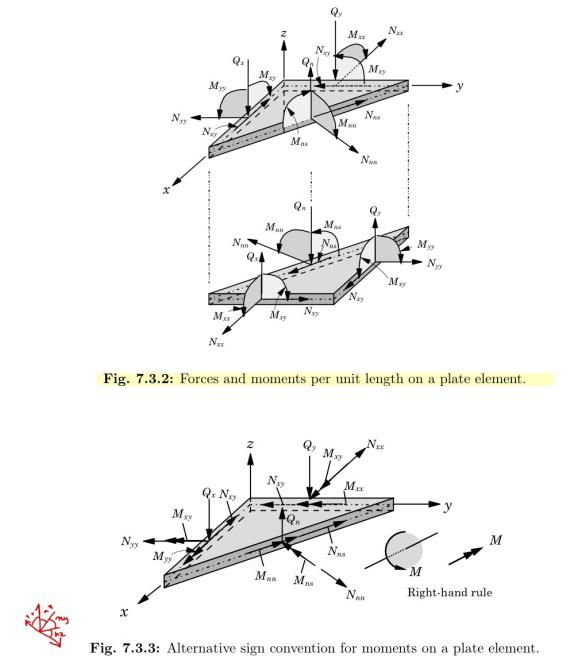
\includegraphics[width=0.6 \linewidth]{\pth/nfem/fig32} 		
		\end{figure}
	\end{frame}


	\begin{frame}
		\begin{itemize}
			\item The virtual work by the distributed transverse load q(x,y), reaction force of an elastic foundation, in plane normal stress $\sigma_{nn}$, in plane tangential stress $\sigma_{ns}$, transverse shear stress $\sigma_{nz}$ is 
			\begin{equation}
			\begin{aligned}
				\delta W_E^e = - (\int_A q(x,y) \delta w(x,y,\frac{h}{2}) dx~dy + 
				\int_A F_s(x,y) \delta w(x,y,-\frac{h}{2}) dx~dy
				\\	+ \int_S \int_{-\frac{h}{2}}^{\frac{h}{2}} \left[ \sigma_{nn} \left(\delta u_n - z \frac{\delta w}{n} \right) + \sigma_{ns} \left(\delta u_s - z \frac{\delta w}{s}\right) 
				+ \sigma_{nz}\delta w\right] dz~ds ) \\ 
				= - \left[ \int_S \left(N_{nn}\delta u_n - M_{nn}\frac{\partial \delta w}{\partial n}
							+ N_{ns}\delta u_s 
				            - M_{ns}\frac{\partial \delta w}{\partial s} + Q_n \delta w \right)ds
				            + \int_A (q-kw)\delta w dx~dy
				 \right] 
			\end{aligned}
			\end{equation}
			\item where Fs = -kw ( Foundation force), the negative sign it is the force applied upwards, but you can think of it like the potential increases as the w increases.
			\item The last term in the work term is the virtual work of the transverse and normal forces on a boundary that is inclined. Where N = $\int_{-\frac{h}{2}}^{\frac{h}{2}}\sigma$ ,  M = $\int_{-\frac{h}{2}}^{\frac{h}{2}}z\sigma$, $Q_n = \int_{-\frac{h}{2}}^{\frac{h}{2}}\sigma_{nz}$ 
		\end{itemize}
	\end{frame}


	\begin{frame}
	\begin{itemize}
		\item We now relate the stresses in the direction in the boundary to the internal stresses given in cartesion using stress tensor coordinate transformation
			\begin{equation}
			   \mat{\sigma_{nn}; \sigma_{ns}} = \mat{n_x^2,n_y^2,2n_xn_y ; -n_xn_y,n_xn_y,n_x^2 - n_y^2} \mat{\sigma_{xx};\sigma_{yy};\sigma_{xy}}
			\end{equation}
	\end{itemize}
	\end{frame}


	\begin{frame}{Weak forms}
		\begin{itemize}
			\item Keeping the weak forms in the full virtual work statement we get
			\begin{equation}
			\tiny
				\begin{aligned}
					0 =  \int_A \left(N_{xx}\delta \varepsilon_{xx}^0 + M_{xx}\delta\varepsilon_{xx}^1 + N_{yy}\delta\varepsilon_{yy}^0 + M_{yy}\delta\varepsilon_{yy}^1 
					+ N_{xy}\delta\gamma_{xy}^0 + M_{xy}\delta\gamma_{xy}^1 \right) dx~dy \\ - \left[ \int_S \left(N_{nn}\delta u_n - M_{nn}\frac{\partial \delta w}{\partial n}
					+ N_{ns}\delta u_s 
					- M_{ns}\frac{\partial \delta w}{\partial s} + Q_n \delta w \right)ds
					+ \int_A (q-kw)\delta w dx~dy
					\right]  \\ 
					 =  \int_A \left(N_{xx}\delta \varepsilon_{xx}^0 + M_{xx}\delta\varepsilon_{xx}^1 + N_{yy}\delta\varepsilon_{yy}^0 + M_{yy}\delta\varepsilon_{yy}^1 
					 + N_{xy}\delta\gamma_{xy}^0 + M_{xy}\delta\gamma_{xy}^1 \right) dx~dy \\ - \left[ \int_S \left(N_{nn}\delta u_n - M_{nn}\frac{\partial \delta w}{\partial n}
					 + N_{ns}\delta u_s 
					 - M_{ns}\frac{\partial \delta w}{\partial s} + Q_n \delta w \right)ds
					 + \int_A (q-kw)\delta w dx~dy
					 \right]  
				\end{aligned}
			\footnote{\tiny In the last three statements, It seems the equation has been kept according to the variation but how do you account for $ \delta u_n \quad \delta u_s$ as they will have components in both. Maybe the euler equations will make sense}
			\end{equation}
			
			\begin{figure}
				\centering
				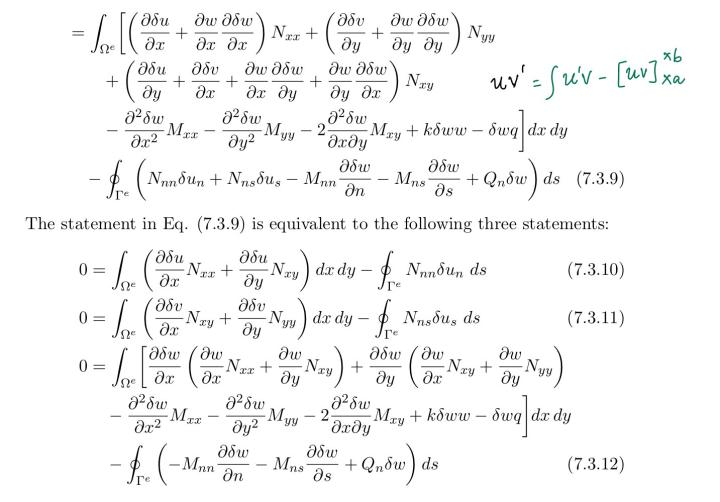
\includegraphics[width=0.6 \linewidth]{\pth/nfem/fig33} 		
			\end{figure}
	
		\end{itemize}
	\end{frame}


	\begin{frame}{Equilibrium equations}
		\begin{itemize}
			\item Keeping the virtual parameters in the same order to get the euler equations we get
			\begin{equation}
			\tiny
			\begin{aligned}
				0 = \int_A \left[ -\left(N_{xx,x} + N_{xy,y}\right)\delta u - \left( N_{xy,x} + N_{yy,y}\right)\delta v
		  			- \left(M_{xx,xx} + 2M_{xy,xy} + M_{yy,yy} + \mathcal{N} - kw + q\right) \delta w
							\right] dx~dy \\
				+ \int_S  (\left(N_{xx}n_x + N_{xy}n_y \right)\delta u  
			  + \left(N_{xy}n_x + N_{yy}n_y \right)\delta v
			  + \left( M_{xx,x}n_x + M_{xy,y}n_x + M_{yy,y}n_y + M_{xy,x}n_y + \mathcal{P} \right) \delta w \\
			  - \left(M_{xx}n_x + M_{xy}n_x \right)\frac{\partial \delta w}{\partial x} 
			  -\left(M_{xy}n_x + M_{yy}n_y \right)\frac{\partial \delta w}{\partial y} )ds  
			  -\int_S \left(N_{nn} \delta u_n + N_{ns}\delta u_s - M_{nn}\frac{\partial \delta w}{\partial n} - M_{ns}\frac{\partial \delta w}{\partial s} + Q_n \delta w \right)ds
			\end{aligned}
			\end{equation}
			\item Where 
				\begin{equation}
				\tiny
					\begin{aligned}
					\mathcal{N} = \frac{\partial }{\partial x} \left(N_{xx}\frac{\partial w}{\partial dx}   + N_{xy}\frac{\partial w}{\partial dy}\right)
					 + \frac{\partial }{\partial y} \left(N_{xy}\frac{\partial w}{\partial x} 
					+ N_{yy}\frac{\partial w}{\partial y}\right) \\
					\mathcal{P} = \left(N_{xx}\frac{\partial w}{\partial x}   + N_{xy}\frac{\partial w}{\partial y}\right) n_x
					+ \frac{\partial }{\partial y} \left(N_{xy}\frac{\partial w}{\partial x} 
					+ N_{yy}\frac{\partial w}{\partial y}\right) n_y 
					\end{aligned}
				\end{equation}
		\end{itemize}
	\end{frame}


	\begin{frame}
		\begin{figure}
			\centering
			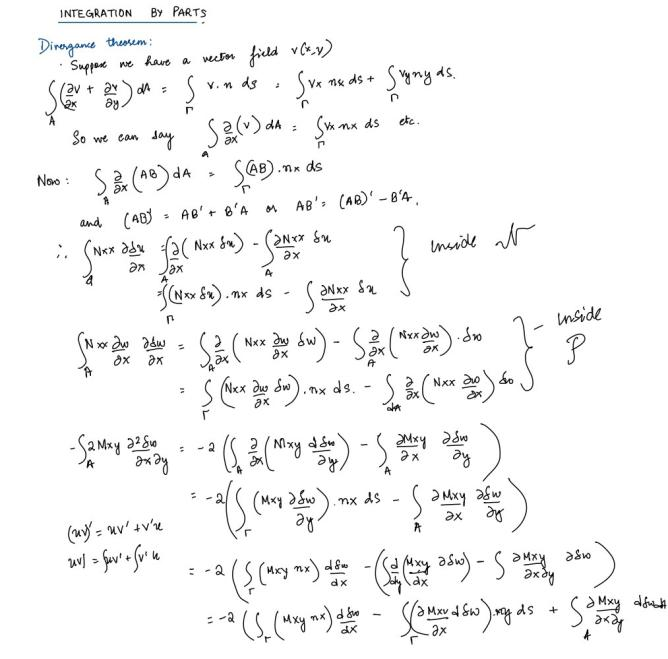
\includegraphics[width=0.7 \linewidth]{\pth/nfem/fig34} 		
		\end{figure}
	\end{frame}


	\begin{frame}{Euler-lagrange equilibrium equations}
		\begin{itemize}
			\item Keeping the coefficients of the variations (seting $\delta u, \delta v, \delta w = 0$)we get the equilibirum equations given as
			\begin{equation}
			\begin{aligned}
				\delta u : \frac{\partial N_{xx}}{\partial x} + \frac{\partial N_{xy}}{\partial y} = 0\\
				\delta v : \frac{\partial N_{xy}}{\partial x} + \frac{\partial N_{yy}}{\partial y} = 0\\
				\delta w : \frac{\partial^2 M_{xx}}{\partial x^2} + 2\frac{\partial^2 M_{xy}}{\partial x \partial y} + \frac{\partial^2 M_{yy}}{\partial y^2} + \mathcal{N} - kw + q = 0
			\end{aligned}
			\end{equation}
		\end{itemize}
	\end{frame}


	\begin{frame}{Boudnary conditions}
		\begin{itemize}
			\item To cast the B.C. on an edge whose normal is $\ve{n}$, we express the generalised displacements ($u,v,w,\frac{\partial w}{\partial x}, \frac{\partial w}{\partial y}$) in x,y,z system in the corresponding displacements in normal, tangential and transverse directions. We get
			\begin{equation}
			\begin{aligned}
				u = u_nn_x - u_sn_y \qquad v = u_nn_y + u_sn_x \\ 
				\frac{\partial w}{\partial x} = \frac{\partial w}{\partial n} n_x 
				- \frac{\partial w}{\partial s}n_y \qquad 
				\frac{\partial w}{\partial y} = \frac{\partial w}{\partial n}n_y
				+ \frac{\partial w}{\partial s}n_x
			\end{aligned}
			\end{equation}
			\begin{figure}
				\centering
				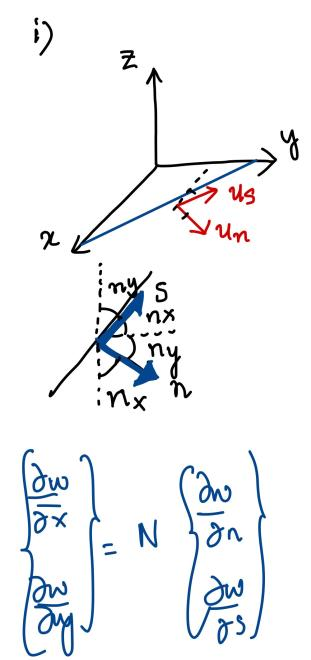
\includegraphics[width=0.2  \linewidth]{\pth/nfem/fig35} 		
			\end{figure}
		Now the derivative of $w$ is a vector which can undergo basis transformation
 		\end{itemize}
	\end{frame}


	\begin{frame}{Boundary conditions}
		\begin{itemize}
			\item The boundary conditions can be written in the normal, tangenetial coords 
			\begin{equation}
			\tiny
			\begin{aligned}
			\int_S [ 
			\left(N_{xx}n_x + N_{xy}n_y\right)\left(\delta u_nn_x - \delta u_sn_y\right) +
			\left(N_{xy}n_x + N_{yy}n_y\right)\left(\delta u_nn_y + \delta u_sn_x\right) \\ +
			\left( M_{xx,x}n_x + M_{xy,y}n_x + M_{yy,y}n_y + M_{xy,x}n_y + \mathcal{P} \right) \delta w \\ - 
			\left(M_{xx}n_x + M_{xy}n_y \right)\left(\frac{\partial w}{\partial n} n_x 
			- \frac{\partial w}{\partial s}n_y \right) - 
			\left(M_{xy}n_x + M_{yy}n_y \right)\left(\frac{\partial w}{\partial n} n_y 
			+ \frac{\partial w}{\partial s}n_x \right)]ds\\
			 - \int_S \left(N_{nn} \delta u_n + N_{ns}\delta u_s - M_{nn}\frac{\partial \delta w}{\partial n} - M_{ns}\frac{\partial \delta w}{\partial s} + Q_n \delta w \right)ds
			\end{aligned} 
			\end{equation}
			\item $\delta u$ in natural does not change the direction cosines because here they are constant dependant on the geometry we are at and not the variation.
		\end{itemize}
	\end{frame}


	\begin{frame}{Boundary conditions}
		\begin{figure}
			\centering
			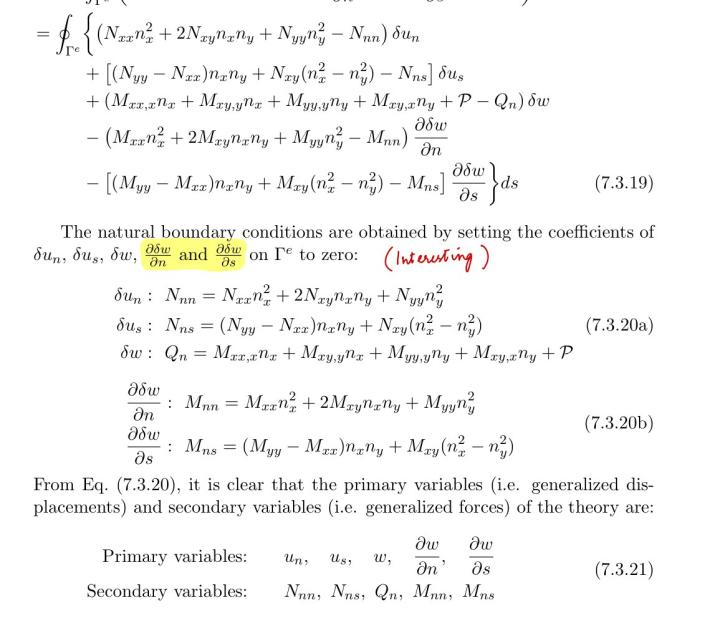
\includegraphics[width=0.7\linewidth]{\pth/nfem/fig36} 		
		\end{figure}
	\end{frame}